\documentclass[14pt]{extarticle}

%%%% paramètres généraux
%%%% french character
\usepackage[french]{babel}
\usepackage[T1]{fontenc}
\usepackage[utf8]{inputenc}

%%%% useful packages
\usepackage[a4paper, left=1.3cm, right=1.3cm, top=2.2cm, bottom=2.3cm]{geometry}
\usepackage{subcaption} % for figure caption
\usepackage{graphicx} % image
\usepackage{tabularx} % table
\usepackage[table]{xcolor} % color in table
\usepackage{amsmath} % math
\usepackage{amssymb} % bold math
\usepackage{wasysym} % integral
\usepackage[many]{tcolorbox} % colored box
\usepackage{fancyhdr} % headers
\usepackage{enumitem} % for bullet in itemize
\usepackage[colorlinks=true,linkcolor=black,citecolor=black,filecolor=black,urlcolor=black]{hyperref} % for link
\usepackage{accents} % for complex notation
\usepackage[european, straightvoltages, RPvoltages]{circuitikz} % for electronic circuit
\usepackage{multicol} % to use several columns
\usepackage{fontawesome} % awesome icons
\usepackage{ifthen} % for loop and boolean in commands
\usepackage{pdfpages} % to include pdf
\usepackage{wrapfig} % to wrap text around figures
\usepackage{chemfig} % to draw chemistry formula
\usepackage{multirow} % for vertically merged cells
\usepackage{makecell} % to format cell in tables
\usepackage{physics} % for derivatives, braket, etc.
\usepackage{esvect} % for large vectors
\usepackage{listings} % for code
\usepackage{dashundergaps} % for automatic text to fill
\usepackage{tabularray} % for better tables
% dyslexia friendly font (need to be compiled in xetex)
%\usepackage{fontspec}
%\setmainfont{OpenDyslexic}


%%%% settings
\setlength{\parskip}{0cm}
\setlength{\parindent}{0cm}
\renewcommand{\baselinestretch}{1}
\setcounter{tocdepth}{2}


%%%% tikz configuration
\usetikzlibrary{babel}
\tikzset{>=latex}


%%%% header
\renewcommand{\headrulewidth}{0.4pt}
\setlength{\headheight}{22.50113pt}


%%%% Table
\renewcommand{\tabularxcolumn}[1]{m{#1}}
\setlength{\extrarowheight}{8pt}


%%%% Chemfig configuration
\setchemfig{
  atom sep=20pt,
  bond style={line width=1pt},
  angle increment=30
}


%%%% dashundergaps configuration
\dashundergapssetup{
  gap-numbers = false,
  gap-format = dot,
  gap-widen,
  gap-extend-percent
}

%%%% quelques commandes
%%%%%%%%%%%%%%%%%%%%%%%%%%%%%%%%%%%%%%%%%%%%%%%%%%%%%%%%%%%%%%%%%%%%%%%%%%
%% rectangle coloré
\NewDocumentCommand{\rectangle}{O{couleurPrim} m m}{%
  \shorthandoff{;}
  \tikz \node (rect) [draw, fill, color=#1,
              minimum width=#2,
              minimum height=#3] {};
  \shorthandon{;}
}

%%%%%%%%%%%%%%%%%%%%%%%%%%%%%%%%%%%%%%%%%%%%%%%%%%%%%%%%%%%%%%%%%%%%%%%%%%%
%%
\tcbset{
  boite cassable/.style = {
    breakable, enhanced jigsaw, % pour s'étendre sur plusieurs pages
  },
  %
  couleur fond/.style = {
    colback = #1, % fond blanc
    colbacktitle = #1, % fond pour le titre blanc
  },
  %
  titre sans separation/.style = {
    couleur fond = white,
    coltitle = black, % couleur du titre
    colframe = couleurSec-800, % couleur de la boite
    boxrule = #1, arc = 0.5mm, % largeur et arrondi des traits de la boite
    titlerule = 0mm, top = 0mm, % pour ne pas avoir de séparation titre/boite
    fonttitle = \bfseries\sffamily, % titre en gras et sans serif
  },
  %
  boite pleine/.style = {
    frame hidden, sharp corners, boxrule = 0mm, % pas de contours
    colback = #1, % fond
  },
  %
  titre sans boite/.style = {
    empty, % pas de boite automatique
    fonttitle = \bfseries\sffamily, coltitle = black, % paramètre du titre
    attach boxed title to top left = {yshift=-2.5mm}, % position
    boxed title style = {empty, size = small, top = 1mm, bottom = 0.5mm},
    title = #1,
  },
}

%% une simple boite vide
\newtcolorbox{boite}[1][]{
  boite cassable, colback = white, top = 4pt,
  #1
}

%%%% Boite colorée avec 
% \begin{boiteColoree}{couleur} contenu \end{boiteColoree}
\newtcolorbox{boiteColoree}[2][]{
  boite cassable, boite pleine = #2,
  #1
}

%%%% Boite pour les documents des activités, avec le format suivant
% \begin{doc}{titre}{label} contenu \end{doc}
\newcounter{documentNum}
\newtcolorbox{doc}[3][]{
  boite cassable,
  titre sans separation = 0.5mm,
  before title = {\refstepcounter{documentNum}},
  title = {Document \arabic{documentNum} -- #2\strut \label{#3}},
  #1
}

%%%% Boîtes pour les activités et TP pour une séquence en plan de travail
% Boite pour afficher la durée recommandée en bas à gauche
\newtcbox{\dureeActivite}[1][]{
  arc = 2mm, % courbes des bords
  colback = couleurTer, colframe = white, % couleurs boite
  coltext = white, % couleur texte
}
% Boite de base pour les activités ou TP, avec le format suivant 
% \begin{boiteActivite}{titre activité}{durée}{label}{compteur}{format titre}
%   contenu
% \end{boiteActivite}
\newtcolorbox{boiteActivite}[6][]{
  boite cassable,
  titre sans separation = 0.5mm,
  before title = {\refstepcounter{#5}},
  title = {#6 \arabic{section}.\arabic{#5} -- #2\strut \label{#4}},
  enlarge bottom by = 12pt,
  overlay= {
    \node at ([xshift = -36pt, yshift = -6pt] frame.south east) {
      \dureeActivite{
        {\small \important[white]{#3}}
      }
    };
  }, % affiche la durée de l'activité dans une petite boite
  remember as = #4,
  #1
}

% Boite pour les activités/TP en plan de travail.
% \begin{activite ou TP}{titre activité}[durée]{label} ; durée = 1h acti, 2h TP par défaut
%   contenu
% \end{activite ou TP}
\NewDocumentEnvironment{activite}{m O{1 h} m}{%
  \begin{boiteActivite}{#1}{#2}{#3}
    {activiteNum}{\documentaire* \hspace{-4pt} Activité}
}{
  \end{boiteActivite}
}
% Compteur pour les TP
\newcounter{TPNum} 
\NewDocumentEnvironment{TP}{m O{2 h} m}{%
  \begin{boiteActivite}{#1}{#2}{#3}
    {TPNum}{\mesure* \hspace{-4pt} TP}
}{
  \end{boiteActivite}
}
% Pour réferencer une activité
\newcommand{\reference}[1]{\arabic{section}.\ref{#1}}

% Boîte pour la tâche finale
\newtcolorbox{tacheFinale}[1][]{
  boite cassable,
  titre sans separation = 0.5mm,
  title = {Tâche finale}, % titre
  #1
}

% Boîte pour l'organisation des séances
\newcounter{seanceNum}
\newtcbox{\seance}[2][]{
  boite cassable,
  titre sans separation = 0.5mm,
  before title = {\refstepcounter{seanceNum}},
  title = {Séance \arabic{seanceNum} \hfill (#2)}, % titre,
  halign=center, valign=center, % pour centrer le contenu
  height = 0.13\textheight, % hauteur de la boite
  #1
}
% Pour afficher 3/2/1 séances dans la programmation
\NewDocumentEnvironment{programmeSeance}{O{3} D(){34}}{
  \begin{tcbraster}[
    raster columns = #1, 
    raster width center = (\linewidth - 3cm - 5cm*(3 - #1))
  ]
}{
  \end{tcbraster}
  \vspace*{#2 pt}
}


%%%% Passage important à connaître
\newtcolorbox{importants}[1][]{
  boite cassable,
  boite pleine = couleurPrim-50, % fond
  shadow = {-4pt}{0mm}{0mm}{couleurPrim}, % barre gauche
  #1
}

%%%% Boîte pour le contexte
\newtcolorbox{contexte}[1][]{
  boite cassable, 
  titre sans separation = 3pt,
  couleur fond = couleurPrim-50!50, 
  colframe = couleurPrim, sharp corners, %  contours
  title = {Contexte :}, % titre
  detach title, before upper={\vspace{2pt}\hspace{-8pt}\tcbtitle\;}, % titre "en ligne"
  #1
}

%%%% Pour les objectifs
\newenvironment{objectifs}{ %
  \begin{listeObjectifs}
} {\end{listeObjectifs}}
%
\tcolorboxenvironment{objectifs}{
  titre sans boite = {Objectifs :},
  frame code = { % tracé de la boite
    \path [draw=couleurPrim, line width = 3pt]
    (frame.west) |- ([xshift=6mm] title.north east)
    to[out=0, in=180] ([xshift=20mm] title.east) -| % définit la courbe
    (frame.east) |- (frame.south) -| cycle; % trace la boite
  },
}

%% Pour les pré-requis
\newenvironment{prerequis}{ %
  \begin{listeObjectifs}
} {\end{listeObjectifs}}
%
\tcolorboxenvironment{prerequis}{
  titre sans boite = {Prérequis :},
  frame code = { % tracé de la boite
    \path [draw=couleurPrim, line width = 3pt]
    (frame.south east) |- ([xshift=-34mm, yshift=-4mm] frame.south east)
    to[out=180, in=0] ([xshift=-47mm] frame.south east) -| % définit la courbe
    (frame.west) |- (title.north) -| cycle; % trace la boite
  },
}

%%%% Espace pour un coup de pouce
\newcounter{coupDePouceNum}
\newtcolorbox{coupDePouce}[1][]{
  boite cassable, 
  titre sans separation = 0.5mm,
  before title = {\refstepcounter{coupDePouceNum}},
  title = {
    \textcolor{couleurPrim}{\faThumbsUp}
    Coup de pouce \arabic{coupDePouceNum} :
    \flushright \vspace*{-24pt}\faSquareO
  },
  #1
}

%%%% Espace pour une appréciation
\newcommand{\appreciation}[1]{
  \pasCorrection{
    \begin{boite}
      \vspace*{-4pt}
      \important[black]{Appréciation et remarques}
      \vspace*{#1 cm} \phantom{b}
    \end{boite}
  }
}

%%%% Espace fiche TP
\newtcolorbox{boiteMateriel}[2][]{
  titre sans separation = 0.5mm,
  coltitle = white, colbacktitle = couleurPrim, % fond pour le titre blanc
  title = {\centering \large \phantom{À} #2 \phantom{g}}, % titre
  #1
}

%%%%%%%%%%%%%%%%%%%%%%%%%%%%%%%%%%%%%%%%%%%%%%%%%%%%%%%%%%%%%%%%%%%%%%%%%%
%%%% pagination et sections
\NewDocumentCommand{\titre}{O{black} m}{
  \begin{center}
    \textcolor{#1} {\textsf{\bfseries \Large #2}}
  \end{center}
}
\newcommand{\pasDePagination}{
  \thispagestyle{empty}
}
\newcommand{\feuilleBlanche}{
  \newpage
  \phantom{b}
  \pasDePagination
}
\NewDocumentCommand{\inclusActivite}{O{1} m}{
  \numeroActivite{#1}
  \input{#2}
}
    

%%%% activité ou TP
\newcounter{activiteNum}
\newcommand{\titreActi}[2]{
  \refstepcounter{activiteNum}
  \titre{#1 \arabic{section}.\arabic{activiteNum} -- #2}
}
\NewDocumentCommand{\titreTP}{s m}{
  \IfBooleanTF{#1}{ % Version *
    \titreActi{Activité expérimentale}{#2}
  }{
    \titreActi{TP}{#2}
  }
}
\NewDocumentCommand{\titreActivite}{s m O{Activité}}{
  \IfBooleanTF{#1}{ % Version * sans le numéro du chapitre
    \refstepcounter{activiteNum}
    \titre{#3 \arabic{activiteNum} -- #2}
  }{
    \titreActi{#3}{#2}
  }
}
\NewDocumentCommand{\titreEvaluation}{o m}{
  \IfNoValueTF{#1}{
    \titre{Évaluation \arabic{section} -- #2}
  }{
    \titre{Évaluation #1 -- #2}
  }
  % reinitialisation du numéro de page et d'exercices
  \reinitialiseCompteur
}
\newcounter{exerciceNum}
\newcommand{\exercice}[1]{
  \refstepcounter{exerciceNum}
  \important[black]{\large Exercice \arabic{exerciceNum} : #1}
  % reset des numéros de questions
  \setcounter{questionNum}{0}
  \setcounter{documentNum}{0}
}


%%%% chapitre, partie, section et sous-section
\newcommand{\chapitre}[1]{ % Réglage du titre du chapitre
  Chapitre \arabic{section} -- #1
}
\newcommand{\titreChapitre}[1]{ % Affichage du titre du chapitre
  \titre{Chapitre \arabic{section} -- #1}
}
\newcommand{\titrePartie}[1]{
  \vspace*{24pt}
  \refstepcounter{subsection}
  \rectangle{40pt}{1pt}
  \important[black]{\Large \Roman{subsection} -- #1}
  \rectangle{40pt}{1pt}
  \vspace*{10pt}
}
\newcounter{sousSectionNum}
\newcommand{\titreSection}[1]{
  \vspace*{16pt}
  \refstepcounter{subsubsection}
  \setcounter{sousSectionNum}{0}
  \rectangle{30pt}{4pt}
  \important[black]{\large \arabic{subsubsection} -- #1}
  \vspace*{4pt}
}
\newcommand{\titreSousSection}[1]{
  \vspace*{12pt}
  \refstepcounter{sousSectionNum}
  \important[black]{\Alph{sousSectionNum} -- #1}
  \vspace*{4pt}
}

%%%% fixe le numéro de l'activité
\newcommand{\reinitialiseCompteur}{
    % fixe les compteurs LaTeX
  \setcounter{subsection}{0}
  \setcounter{subsubsection}{0}
  \setcounter{figure}{0}
  % fixe les compteurs internes
  \setcounter{documentNum}{0}
  \setcounter{questionNum}{0}
  \setcounter{coupDePouceNum}{0}
  \setcounter{sousSectionNum}{0}
  \setcounter{seanceNum}{0}
}
\newcommand{\numeroActivite}[1]{
  \reinitialiseCompteur
  \setcounter{activiteNum}{#1 - 1}
}
% fixe le numéro de partie (#1) et le numéro de la page (#2)
\newcommand{\numeroPartieCours}[2]{
  \newpage
  \setcounter{subsection}{#1 - 1}
  \setcounter{page}{#2}
}

%%%% lignes
\newcommand{\ligne}{
  \par\noindent\rule{\textwidth}{0.4pt}
}
\NewDocumentCommand{\lignePointillee}{o}{
  \IfValueTF{#1}{
    \makebox[#1\linewidth]{\dotfill}
  }{
    \phantom{b}\hspace*{-12pt} \dotfill
  }
}


%%%%%%%%%%%%%%%%%%%%%%%%%%%%%%%%%%%%%%%%%%%%%%%%%%%%%%%%%%%%%%%%%%%%%%%%%%
%%%% Paramètre par défaut pour l'en-tête
\newcommand{\classe}{Réglez avec \textbackslash renewcommand\{\textbackslash classe\}\{Seconde\}}
\newcommand{\etablissement}{Réglez avec \textbackslash renewcommand\{\textbackslash etablissement\}\{Lycée\}}

%%%% en-tête
\newcommand{\teteGauche}[2]{
  \lhead{
    \textbf{\footnotesize #1}
    \newline
    \footnotesize #2
  }
}
\NewDocumentCommand{\teteDroite}{m o}{
  \rhead{
    \IfValueT{#2}{
      \hfill \textbf{\footnotesize #2}
    }
    \newline 
    \hfill \footnotesize #1
  }
}
%% \enTete [compteur] {titre} [numéro de section] ; * = version simplifié sans pagination
\NewDocumentCommand{\enTete}{s o m O{0}}{
  % reset des compteurs
  \newpage
  \reinitialiseCompteur
  \setcounter{section}{#4}
  
  \IfBooleanTF{#1}{ % affichage de l'entête version fiche réussite (*)
    \pasDePagination
    \phantom{b} \vspace*{-70pt}
    \titre{#3}
  }{ % affichage de l'entête version activité
    \pagestyle{fancy}
    \teteGauche{\etablissement{}}{#3} % left header
    \chead{} % central header
    \teteDroite{#2} % right header
  }
}


%%%%%%%%%%%%%%%%%%%%%%%%%%%%%%%%%%%%%%%%%%%%%%%%%%%%%%%%%%%%%%%%%%%%%%%%%%
%%%% exercice
% définit un booléen pour entrer ou sortir du mode correction
\newboolean{modeProf}
\setboolean{modeProf}{false}
\newcommand{\modeCorrection}{
  \setboolean{modeProf}{true}
  \TeacherModeOn
}

%% Affiche le numéro d'une question avec choix du compteur et de l'espacement
\NewDocumentCommand{\numeroQuestion}{s O{questionNum} O{16}}{
  \refstepcounter{#2}
  \setcounter{sousQuestionNum}{0}
  \vspace*{2pt}
  \IfBooleanTF{#1}{}{ % cas non étoilé
    \ifnum \thequestionNum > 9
      \hspace{6 pt}
    \else
      \hspace{#3 pt}
    \fi
  }
  \textcolor{couleurSec}{
    \textbf{\arabic{#2}} {\small\faMinus}
  }
}
%% Sous question sour la forme 1.2
\NewDocumentCommand{\numeroSousQuestion}{O{16}}{
  \refstepcounter{sousQuestionNum}
  \ifnum \thesousQuestionNum > 9
    \hspace{6 pt}
  \else
    \hspace{#1 pt}
  \fi
  \textcolor{couleurSec}{
    \textbf{\arabic{questionNum}.\arabic{sousQuestionNum}.}
  }
}


%% trace des lignes pointillées pour répondre aux questions
% \lignesDeReponse* complète la ligne actuelle par des pointillées
% \lignesDeReponse commence à la ligne suivante
\newcounter{ligneNum}
\NewDocumentCommand{\lignesDeReponse}{s m}{
  % Trace la fin de la ligne, ou pas
  \IfBooleanTF{#1}{ % Version *
    \espaceReponse \dotfill\phantom{bb}
    \ifnum #2 < 1
      \newline
    \fi
  }{}
  % Trace le bon nombre de lignes
  \setcounter{ligneNum}{-1}
  \loop
    \stepcounter{ligneNum}
    \ifnum \value{ligneNum} < #2
      \\[8pt] \lignePointillee
  \repeat
  \vspace*{1pt}
}


%% définit une commande pour afficher une question 
% \qestion {question} {réponse} [nombre de lignes] ; * = pas d'alinéa
\newcounter{questionNum}
\newcounter{sousQuestionNum}
\NewDocumentCommand{\question}{s +m +m O{0}}{
  \IfBooleanTF{#1}{ % étoile
    \numeroQuestion* \!#2
  }{ % 
    \numeroQuestion \!#2
  }
  % pointille ou correction
  \ifthenelse {\boolean{modeProf}} { % prof
    \begin{boiteColoree}{couleurPrim-50}
      #3
    \end{boiteColoree}
  }{ % eleve
    \lignesDeReponse{#4}
  }
}

% Affiche le contenu en mode correction
\newcommand{\correction}[1]{
  \ifthenelse {\boolean{modeProf}} { % correction
    #1
  }{}
}

% Affiche le contenu si on est pas en mode correction
\newcommand{\pasCorrection}[1]{
  \ifthenelse{\boolean{modeProf}} {}{ % pas correction
    #1
  }
}

% Point associé à une question
\newcommand{\points}[1]{
  \marginnote{#1}
}


% sous questions
\newcommand{\sousQuestion}[2]{
  \hspace{16pt}
  \textcolor{couleurSec}{\textbullet} #1
  
  \vspace*{8pt}
  \reponse{#2}
}

%%%% qcm
\newlist{QCM}{itemize}{2}
\setlist[QCM]{label = $\square$, leftmargin = 2cm}
%% #1 : question, 
%% #2 : réponses
\NewDocumentEnvironment{qcm}{+m +m}{
  \numeroQuestion #1
  \begin{QCM}
    #2
}{
  \end{QCM}
}

% À ajouter devant la bonne réponse dans un qcm
\newcommand{\reponseQCM}{
  \correction{
    \hspace*{-21pt}
    {\large\textcolor{couleurSec}{\faCheck}}
    \hspace*{-12pt}
  } % Note : trace une croix à la bonne position
}

%%%% Pour afficher les compétences
\newcommand{\competence}[1]{
  ~{\footnotesize\textit{(#1)}}
}

%%%% Espace pour indiquer nom, prénom et classe
\newcommand{\nomPrenomClasse}{
  \pasCorrection{
    \vspace*{-24pt}
    Nom : \lignePointillee[0.3]
    Prénom : \lignePointillee[0.3]
    Classe : \dotfill
  }
}
\newcommand{\nomPrenom}{
  \pasCorrection{
    \vspace*{-24pt}
    Nom : \lignePointillee[0.3]
    Prénom : \lignePointillee[0.3]
  }
}


%%%%%%%%%%%%%%%%%%%%%%%%%%%%%%%%%%%%%%%%%%%%%%%%%%%%%%%%%%%%%%%%%%%%%%%%%%
% texte à trou avec option pour régler la largeur
\NewDocumentCommand{\texteTrou}{s o +m}{
  \ifthenelse {\boolean{modeProf}}{ % prof
    \IfBooleanTF{#1}
    {#3}
    {\important[black]{#3}}
  }{ % élève
    \IfValueTF{#2}{ % Si la largeur est réglée, on utilise des lignes
      \espaceReponse
      \lignePointillee[#2]
      \hspace*{-12pt}
    }{ % Sinon on utilise dash undergap pour la version automatique
      \espaceReponse \hspace*{0.1pt}
      \gap{#3}
    }
  }
}

% texte à trou avec option pour laisser plusieurs lignes
\NewDocumentCommand{\texteTrouLignes}{O{0} +m}{
  \ifthenelse {\boolean{modeProf}} {% prof
    \important[black]{#2}
  }{% élève
    \lignesDeReponse*{#1}
  }
}

% espace vertical pour la réponse
\newcommand{\espaceReponse}{
  \phantom{$\dfrac{1}{1}$} % espace vertical
  \hspace*{-38pt} \phantom{b} % ajuste l'espace horizontal
}


%%%%%%%%%%%%%%%%%%%%%%%%%%%%%%%%%%%%%%%%%%%%%%%%%%%%%%%%%%%%%%%%%%%%%%%%%%
%%%% Pour choisir parmi deux sujets
\newboolean{sujetA}
\setboolean{sujetA}{true}
\newcommand{\sujetB}{
  \setboolean{sujetA}{false}
}
\newcommand{\sujetA}{
  \setboolean{sujetA}{true}
}

%%%% Pour faire plusieurs sujets en parallèle
\newcommand{\variationSujet}[2]{
  \hspace*{-6pt}
  \ifthenelse{\boolean{sujetA}}{#1}{#2}
  \hspace*{-6pt}
}


%%%%%%%%%%%%%%%%%%%%%%%%%%%%%%%%%%%%%%%%%%%%%%%%%%%%%%%%%%%%%%%%%%%%%%%%%%
%%%% Tableau générique avec la première ligne bleue
\NewDocumentEnvironment{tableau}{m}{
  \begin{center}
    \begin{tblr}{
      hlines,
      colspec = #1,
      row{1} = {couleurSec-100},
    }
}{
    \end{tblr}
  \end{center}
}

%%%% Tableau de competence
\newenvironment{tableauCompetences}{
  \begin{center}
    \begin{tblr}{
      colspec = {c X[l] c c c c},
      rows = {m}, hlines, vlines,
      row{1} = {c, couleurSec-100, font = \bfseries}
    }
      Comp. & Items & D & C & B & A \\
}{
    \end{tblr}
  \end{center}
}

%%%% Tableau de connaissances pour les fiches de révisions
\newenvironment{tableauConnaissances}{
  \begin{center}
  \begin{tblr}{
    colspec = {Q[t, wd=0.7\textwidth] c c c},
    rows = {m}, hlines, vlines,
    column{4} = {0.2},
    row{1} = {couleurSec-100, c}
  }
    \important{Connaissances et capacités exigibles} & \ok & \pasOk & \important{En classe} \\
}{ 
  \end{tblr}
  \end{center}
}

%%%% Tableau de mémorisation pour les fiches de mémorisation
% Question | | | Réponse
\newenvironment{tableauMemorisation}{
  \begin{center}
 \begin{tblr}{
    colspec = {
      Q[l, wd=0.3\textwidth] % Question
      X[c] X[c] % Auto-évaluation
      Q[l, wd=0.3\textwidth] % Réponse
      Q[c, wd=0.045\textwidth] Q[c, wd=0.045\textwidth] Q[c, wd=0.045\textwidth] % Répétitions
    }, rows = {m}, hlines, vlines,
    row{1,2} = {couleurSec-100, c}
  }
    \SetCell[r=2]{c} \important{Questions} & 
    \SetCell[c=2]{c} \important{Auto-évaluation} & &
    \SetCell[r=2]{c} \important{Réponses} & 
    \SetCell[r=2]{c} \important{J-7} &
    \SetCell[r=2]{c} \important{J-30} &
    \SetCell[r=2]{c} \important{J-180} \\
    %
    & % questions
    \ok & \pasOk & % auto evaluation
    & % réponses 
    & & \\ % répétitions
    %
}{ 
  \end{tblr}
  \end{center}
}


%%%% Alignement vertical dans un tableau
\newcommand{\vAligne}[1]{
  \strut \\ \vspace*{#1}
}


%%%%%%%%%%%%%%%%%%%%%%%%%%%%%%%%%%%%%%%%%%%%%%%%%%%%%%%%%%%%%%%%%%%%%%%%%%
%%%% symboles : chevron, flèche, attention, etc.
\NewDocumentCommand{\chevron}{O{couleurPrim}}{
  \textcolor{#1}{\small \faChevronRight}
}
%
\NewDocumentCommand{\fleche}{O{couleurPrim}}{
  \textcolor{#1}{\faCaretRight}
}
%
\NewDocumentCommand{\attention}{O{couleurPrim}}{
  \textcolor{#1}{\faExclamationTriangle}
}
%
\NewDocumentCommand{\flecheLongue}{O{couleurPrim}}{
  \textcolor{#1}{\faLongArrowRight}
}
%
\NewDocumentCommand{\ok}{O{couleurPrim}}{
  \textcolor{#1}{\faCheckCircle}
}
%
\NewDocumentCommand{\pasOk}{O{couleurPrim}}{
  \textcolor{#1}{\faTimesCircle}
}
%
\NewDocumentCommand{\pointCyan}{O{couleurPrim}}{
  \textcolor{#1}{\textbullet}
}

%% Commande générale pour colorer un texte avec une couleur par défaut
% L'intérêt de cette commande est d'éviter des répétion de O{couleurSec}
\NewDocumentCommand{\questionSpeciale}{O{couleurSec} m}{
  \textcolor{#1}{#2}
}
% Quelques questions spéciales avec couleur réglable et un espace horizontal
\NewDocumentCommand{\mesure}{s o}{
  \IfBooleanTF{#1}{}{ \hspace{7pt} }
  \questionSpeciale[#2]{\faFlask\hspace{1pt} \faWrench\!}
}
%
\NewDocumentCommand{\telechargement}{s o}{
  \IfBooleanTF{#1}{}{ \hspace{7pt} }
  \questionSpeciale[#2]{\faDownload\, \faMobile\;}
}
%
\NewDocumentCommand{\documentaire}{s o}{
  \IfBooleanTF{#1}{}{ \hspace{7pt} }
  \questionSpeciale[#2]{\faFileText\hspace{1pt} \faBook}
}

%% pictogramme de sécurité \picto {largeur} {pictogramme}
\newcommand{\picto}[2]{
  \image{#1}{images/pictogrammes/picto_#2}
}
% Nombre dans un cercle A REVOIR
\newcommand*\nombreCercle[1]{
  % \tikz[baseline=(char.base)]{
  %   \node [shape=circle, draw filled, inner sep=1.2pt, color=couleurSec-50] (char) {\textcolor{black}{#1};
  % }
  \important[couleurSec]{#1}
}
% Pour légender une image
\newcommand{\legende}[1]{
  \vspace*{4pt}
  \textcolor{couleurPrim}{\faArrowUp} \; #1
}

%%%%%%%%%%%%%%%%%%%%%%%%%%%%%%%%%%%%%%%%%%%%%%%%%%%%%%%%%%%%%%%%%%%%%%%%%%
%%%% points importants
\NewDocumentCommand{\important}{O{couleurSec-800} +m}{
  \!\textcolor{#1}{\textsf{\bfseries #2}}\!\!
}
%%%% Pour donner des exemples. 
% \exemple est au singulier, \exemple* est au pluriel.
\NewDocumentCommand{\exemple}{s}{
  \fleche
  \IfBooleanTF{#1}{
    \textit{Exemples :}
  }{
    \textit{Exemple :}
  }
}

%%%% Citation (#1) avec la source (#2)
\newcommand{\extrait}[2]{
  « #1 »
  
  \vspace*{-12pt}
  \begin{flushright}
    \textit{#2}
  \end{flushright}
  \vspace*{-12pt}
}

%%%% image avec la largeur réglée par rapport à celle de la ligne
\newcommand{\image}[2]{
  \includegraphics[width=#1\linewidth]{#2}
}

%%%% qr code en insert sur la droite
\NewDocumentCommand{\qrcodeCote}{o +m D(){-16pt} O{1.5cm}}{
  \IfNoValueTF{#1} {
    \begin{wrapfigure}{r}{0.1\linewidth}
      \vspace*{#3}
      \qrcode[height = #4]{#2}
    \end{wrapfigure}
  }{
    \begin{wrapfigure}[#1]{r}{0.1\linewidth}
      \vspace*{#3}
      \qrcode[height = #4]{#2}
    \end{wrapfigure}
  }
}


%%%%%%%%%%%%%%%%%%%%%%%%%%%%%%%%%%%%%%%%%%%%%%%%%%%%%%%%%%%%%%%%%%%%%%%%%%
%%%% protocole, avec plusieurs colonnes possibles
\NewDocumentEnvironment{protocole}{o +m}{
  \IfValueTF{#1}{
    \vspace*{-8pt}
    \begin{multicols}{#1}
  }{}
  \begin{itemize}[label = {\footnotesize \fleche[couleurSec]}]
    #2
}{
  \end{itemize}
  \IfValueTF{#1}{ \end{multicols} }{}
}

%%%% liste de points, avec plusieurs colonnes possibles
\NewDocumentEnvironment{listePoints}{o +m}{
  \IfValueTF{#1}{
    \vspace*{-8pt}
    \begin{multicols}{#1}
  }{}
  \begin{itemize}[label = \pointCyan]
    #2
}{
  \end{itemize}
  \IfValueTF{#1}{ \end{multicols} }{}
}

%%%% jeu de données, avec plusieurs colonnes possibles
\NewDocumentEnvironment{donnees}{o +m}{  
  \important{Données :}
  \IfValueTF{#1}{
    \vspace*{-8pt}
    \begin{multicols}{#1}
  }{}
  \begin{listeTirets}
    #2
}{
  \end{listeTirets}
  \IfValueTF{#1}{ \end{multicols} }{}
}

%%%% liste d'objectif
\newlist{listeObjectifs}{itemize}{2}
\setlist[listeObjectifs]{leftmargin=6pt, label=\fleche}

%%%% liste tirets
\newlist{listeTirets}{itemize}{2}
\setlist[listeTirets]{label = \textcolor{couleurPrim}{\small\faMinus}}

%%%% liste avec des flèches
\newlist{listeFleche}{itemize}{2}
\setlist[listeFleche]{label = \textbf{\flecheLongue}}

%%%% liste avec chiffre
\newlist{enumeration}{enumerate}{2}
\setlist[enumeration]{label = \textcolor{couleurSec}{\textbf{\arabic*.}} }

%%%% problématique 
\newcommand{\problematique}[1]{
  \hspace*{-12pt}
  \flecheLongue[couleurTer]
  \hspace*{-10pt}
  \important[couleurTer]{#1}
}


%%%%%%%%%%%%%%%%%%%%%%%%%%%%%%%%%%%%%%%%%%%%%%%%%%%%%%%%%%%%%%%%%%%%%%%%%%
%%%% Séparation de la page en trois blocs
\NewDocumentCommand{\separationTroisBlocs}{+m O{0.3} +m O{0.3} +m O{0.3}}{
  \begin{minipage}[T]{#2\linewidth}
    #1
  \end{minipage}
  ~
  \begin{minipage}[T]{#4\linewidth}
    #3
  \end{minipage}
  ~
  \begin{minipage}[T]{#6\linewidth}
    #5
  \end{minipage}
}
%%%% Separation en deux blocs
\NewDocumentCommand{\separationBlocs}{+m O{0.48} +m O{0.48}}{
  \begin{minipage}[T]{#2\linewidth}
    #1
  \end{minipage}
  \hfill
  \begin{minipage}[T]{#4\linewidth}
    #3
  \end{minipage}
}


%%%%%%%%%%%%%%%%%%%%%%%%%%%%%%%%%%%%%%%%%%%%%%%%%%%%%%%%%%%%%%%%%%%%%%%%%%
%% nombre algébrique et réaction chimique
\newcommand{\algebrique}[1]{
  \ensuremath{\overline{\mathrm{#1}}}
}
\newcommand{\reaction}{
  \;\text{\faLongArrowRight}\; % flèche courte et jolie
}

%% Pour simplifier l'écriture des formules brutes
% #1 : # carbone, #2 : # hydrogène, #3 : oxygène
\newcommand{\bruteCHO}[3]{
  \chemfig{C_{#1} H_{#2} O_{#3}}
}

%% pour les masse molaire et atomique (* -> en indice)
\NewDocumentCommand{\masseMol}{s m}{
  \IfBooleanTF{#1}{
    \ensuremath{M_{\chemfig{#2}}}
  }{
    \ensuremath{M(\chemfig{#2})}
  }
}
\NewDocumentCommand{\masseAtom}{s m}{
  \IfBooleanTF{#1}{
    \ensuremath{m_{\chemfig{#2}}}
  }{
    \ensuremath{m(\chemfig{#2})}
  }
}


%% Unités pour siunit
\DeclareSIUnit{\dioptre}{\text{$\delta$}}
\DeclareSIUnit{\dornic}{\text{\textdegree D}}
\DeclareSIUnit{\ppm}{\text{ppm}}
\DeclareSIUnit{\COeq}{\text{kgCO$_{2}$e}}
\DeclareSIUnit{\jour}{\text{jour}}
% \DeclareSIUnit{}{\text{}}


%%%% atome ou isotope 
%#1: Z, #2: A, #3: X
\makeatletter
\newcommand{\isotope}[3]{%
   \settowidth\@tempdimb{\ensuremath{\scriptstyle#1}}%
   \settowidth\@tempdimc{\ensuremath{\scriptstyle#2}}%
   \ifnum\@tempdimb>\@tempdimc%
       \setlength{\@tempdima}{\@tempdimb}%
   \else%
       \setlength{\@tempdima}{\@tempdimc}%
   \fi%
  \begingroup%
  \ensuremath{
    ^{\makebox[\@tempdima][r]{\ensuremath{\scriptstyle#1}}}
    _{\makebox[\@tempdima][r]{\ensuremath{\scriptstyle#2}}}
    \chemfig{#3}
  }%
  \endgroup%
}%
\makeatother

%% element chimique dans le tableau périodique
\makeatletter
\newcommand{\element}[2]{%
   \settowidth\@tempdimb{\ensuremath{\footnotesize #1}}%
  \begingroup%
  \ensuremath{
    _{\makebox[\@tempdimb][r]{\ensuremath{\small #1}}} 
    \chemfig[atom style={scale=1.3}]{#2}
  }%
  \endgroup%
}%
\makeatother

%% siècle
\newcommand{\siecle}[1]{
  \textsc{\romannumeral #1}\textsuperscript{e}~siècle%
}

%% texte avec une boite autour
\NewDocumentCommand{\texteEncadre}{m O{black}}{
  \textcolor{#2}{
    \frame{
      \vphantom{$\dfrac{1}{1}$} \textcolor{black}{\text{#1}}
    }
  }
}

%% case cochée
\newcommand{\caseCochee}{
  $\text{\rlap{$\checkmark$}}\square$
}


%%%%%%%%%%%%%%%%%%%%%%%%%%%%%%%%%%%%%%%%%%%%%%%%%%%%%%%%%%%%%%%%%%%%%%%%%%
%%%% Style python
\lstdefinestyle{codePython}{
  commentstyle=\color{magenta-500},
  keywordstyle=\color{green-500},
  stringstyle =\color{purple-500},
  numberstyle =\tiny\color{black!50},
  basicstyle  =\ttfamily\footnotesize,
  breakatwhitespace=false, breaklines=true, keepspaces=true,
  showspaces=false, showstringspaces=false, showtabs=false, tabsize=2,
  captionpos=b, numbers=left, numbersep=5pt,
  extendedchars=true,
  literate={é}{{\'e}}1 {è}{{\`e}}1 {à}{{\'a}}1 {°}{{\textdegree}}1 {²}{{$^2$}}1, 
}
\def\inline{\lstinline[style=codePython,language=python]}


%%%%%%%%%%%%%%%%%%%%%%%%%%%%%%%%%%%%%%%%%%%%%%%%%%%%%%%%%%%%%%%%%%%%%%%%%%
%%%% circuit tikz
\NewDocumentCommand{\fixedvlen}{O{0.5cm} m m O{}}{% [semilength]{node}{label}[extra options]
  % get the center of the standard arrow
  \coordinate (#2-Vcenter) at ($(#2-Vfrom)!0.5!(#2-Vto)$);
  % draw an arrow of a fixed size around that center and on the same line
  \draw[-Triangle, #4] ($(#2-Vcenter)!#1!(#2-Vfrom)$) -- ($(#2-Vcenter)!#1!(#2-Vto)$);
  % position the label as in the normal voltages
  \node[anchor=\ctikzgetanchor{#2}{Vlab}, #4] at (#2-Vlab) {#3};
}
%%%% Ce fichier sert à déclarer les titres des chapitres des différents niveaux

%% Commun
\newcommand{\methode} {Outils pratiques}

%% Seconde
%%%% Chapitre
\newcommand{\snd}{Seconde}
\newcommand{\sndCorp} {Corps purs et mélanges}
\newcommand{\sndSolu} {Solutions}
\newcommand{\sndMouv} {Mouvement et interactions}
\newcommand{\sndAtom} {Structure de l'atome}
\newcommand{\sndMole} {Des atomes à la matière}
\newcommand{\sndLumi} {Ondes lumineuses et optique}
\newcommand{\sndTran} {Transformations de la matière}
\newcommand{\sndChim} {Transformations chimiques}
\newcommand{\sndSign} {Signaux et capteurs}

%%%% en-tête correspondant
\newcommand{\teteSndAP}   {\enTete[\snd]{Accompagnement personnalisé}}
\newcommand{\teteSndMeth} {\enTete[\snd]{\chapitre{\methode}}}
\newcommand{\teteSndCorp} {\enTete[\snd]{\chapitre{\sndCorp}}[1]}
\newcommand{\teteSndSolu} {\enTete[\snd]{\chapitre{\sndSolu}}[2]}
\newcommand{\teteSndMouv} {\enTete[\snd]{\chapitre{\sndMouv}}[4]}
\newcommand{\teteSndAtom} {\enTete[\snd]{\chapitre{\sndAtom}}[5]}
\newcommand{\teteSndMole} {\enTete[\snd]{\chapitre{\sndMole}}[6]}
\newcommand{\teteSndLumi} {\enTete[\snd]{\chapitre{\sndLumi}}[3]}
\newcommand{\teteSndTran} {\enTete[\snd]{\chapitre{\sndTran}}[8]}
\newcommand{\teteSndChim} {\enTete[\snd]{\chapitre{\sndChim}}[7]}
\newcommand{\teteSndSign} {\enTete[\snd]{\chapitre{\sndSign}}[9]}


%% Première ST2S
%%%% Chapitres
\newcommand{\premStss}{Première ST2S}
\newcommand{\premStssChim} {Sécurité chimique dans l'habitat}
\newcommand{\premStssVisi} {Propagation de la lumière et vision}
\newcommand{\premStssRedo} {Antiseptique et désinfectant, oxydoréduction}
\newcommand{\premStssLumi} {Les infrarouges et leurs applications}
\newcommand{\premStssOrga} {Structure des molécules organiques}
\newcommand{\premStssBiol} {Molécules d'intérêt biologique}
\newcommand{\premStssBiom} {Biomolécules dans l’organisme}
\newcommand{\premStssRout} {Sécurité routière}
\newcommand{\premStssAlim} {Gestion des ressources naturelles et alimentation}
\newcommand{\premStssElec} {Sécurité électrique dans l'habitat}
\newcommand{\premStssPres} {Propriétés des fluides et pression sanguine}
\newcommand{\premStssSono} {Ondes sonores et audition}

%%%% en-tête
\newcommand{\tetePremStssMeth} {\enTete[\premStss]{\chapitre{\methode}}}
\newcommand{\tetePremStssChim} {\enTete[\premStss]{\chapitre{\premStssChim}}[1]}
\newcommand{\tetePremStssVisi} {\enTete[\premStss]{\chapitre{\premStssVisi}}[2]}
\newcommand{\tetePremStssRedo} {\enTete[\premStss]{\chapitre{\premStssRedo}}[3]}
\newcommand{\tetePremStssLumi} {\enTete[\premStss]{\chapitre{\premStssLumi}}[4]}
\newcommand{\tetePremStssOrga} {\enTete[\premStss]{\chapitre{\premStssOrga}}[5]}
\newcommand{\tetePremStssBiol} {\enTete[\premStss]{\chapitre{\premStssBiol}}[6]}
\newcommand{\tetePremStssRout} {\enTete[\premStss]{\chapitre{\premStssRout}}[7]}
\newcommand{\tetePremStssBiom} {\enTete[\premStss]{\chapitre{\premStssBiom}}[8]}
\newcommand{\tetePremStssAlim} {\enTete[\premStss]{\chapitre{\premStssAlim}}[9]}
\newcommand{\tetePremStssElec} {\enTete[\premStss]{\chapitre{\premStssElec}}[10]}
\newcommand{\tetePremStssPres} {\enTete[\premStss]{\chapitre{\premStssPres}}[11]}
\newcommand{\tetePremStssSono} {\enTete[\premStss]{\chapitre{\premStssSono}}[12]}


%% Terminale ST2S
%%%% Chapitres
\newcommand{\termStss}{Terminale ST2S}
\newcommand{\termStssOrga} {Représentation des molécules organiques}
\newcommand{\termStssAlim} {Sécurité physico-chimique dans l'alimentation}
\newcommand{\termStssImag} {La physique de l'imagerie médicale}
\newcommand{\termStssBiom} {Biomolécules et alimentation}
\newcommand{\termStssMedi} {De la molécule aux médicaments}
\newcommand{\termStssEnvi} {Sécurité chimique dans l'environnement}
\newcommand{\termStssDosa} {Analyser la composition d'un milieu}
\newcommand{\termStssRout} {Sécurité routière}
\newcommand{\termStssCosm} {L'usage responsable des cosmétiques}

%%%% en-tête
\newcommand{\teteTermStssMeth} {\enTete[\termStss]{\chapitre{\methode}}}
\newcommand{\teteTermStssOrga} {\enTete[\termStss]{\chapitre{\termStssOrga}}[1]}
\newcommand{\teteTermStssRout} {\enTete[\termStss]{\chapitre{\termStssRout}}[8]}
\newcommand{\teteTermStssAlim} {\enTete[\termStss]{\chapitre{\termStssAlim}}[2]}
\newcommand{\teteTermStssEnvi} {\enTete[\termStss]{\chapitre{\termStssEnvi}}[6]}
\newcommand{\teteTermStssImag} {\enTete[\termStss]{\chapitre{\termStssImag}}[3]}
\newcommand{\teteTermStssDosa} {\enTete[\termStss]{\chapitre{\termStssDosa}}[7]}
\newcommand{\teteTermStssBiom} {\enTete[\termStss]{\chapitre{\termStssBiom}}[4]}
\newcommand{\teteTermStssMedi} {\enTete[\termStss]{\chapitre{\termStssMedi}}[5]}
\newcommand{\teteTermStssCosm} {\enTete[\termStss]{\chapitre{\termStssCosm}}[9]}


%%%% Paramètres réglable
\colorlet{couleurPrincipale}{cyanSombre}
\colorlet{couleurImportant}{vertSombre}
% \modeCorrection

%%%% TP
\begin{document}
  %%%% Sommative
  %%%% tube à essai de sang
\newcommand{\tubeEssaiSang}[1]{
  \begin{subfigure}{0.1\linewidth}
    \centering
    \begin{tikzpicture}
      \tkzBasTubeEssai{#1}{0.25}{0}{0.75}{0.1}
      \tkzTubeEssai{0.25}{1.5}{0.1}
    \end{tikzpicture}
    \caption{}
  \end{subfigure}
}

%%%% Tube à essai de sang centrifugé
\newcommand{\tubeEssaiSangC}[3]{
  \centering
  \begin{tikzpicture}
    \tkzBasTubeEssai{rougeSombre!75!white}{0.5}{0}{#1}{0.1}
    \tkzPhaseTubeEssai{gray!10!white}{0.5}{#1}{#2}{0.1}
    \tkzPhaseTubeEssai{jauneClair!75!white}{0.5}{#2}{#3}{0.1}
    \tkzLegende{Plasma}{0.5}{#3 - 0.5}{2}
    \tkzLegende{Globules blancs}{0.5}{#2-0.08}{2}
    \tkzLegende{Globules rouges}{0.5}{-0.1}{2}
    \tkzTubeEssai{0.5}{#3 + 1}{0.1}
  \end{tikzpicture}
  \caption{}
}


%%%%
\newcommand{\VEth}{V_\text{éth}}
\newcommand{\mEth}{m_\text{éth}}
\newcommand{\rhoEth}{\rho_\text{éth}}
\newcommand{\cEth}{c_\text{éth}}
\newcommand{\COeq}{kg\chemfig{CO_2}e\;}
  %%%% Evaluation 1 : corps pur et mélanges
\newcommand{\competenceEvaluationUn}{
  \begin{tableauCompetences}
    \centering RCO &
    Restituer ses connaissances.
    & & & & \\
    %
    \centering APP &
    Extraire une information.
    & & & &  \\
    %
    \centering VAL &
    Comparer avec des valeurs de références.
    & & & & \\
    %
    \centering ANA/RAI &
    Interpréter des mesures.
    & & & & \\
    %
    \centering REA &
    Réaliser un calcul.
    & & & & \\
  \end{tableauCompetences}
}


%%%% Evaluation 2 : solution
\newcommand{\competenceEvaluationDeux}{
  \begin{tableauCompetences}
    \centering RCO &
    Restituer ses connaissances.
    & & & & \\
    %
    \centering APP &
    Extraire une information, analyser un document.
    & & & & \\
    %
    \centering VAL &
    Comparer avec des valeurs de références.
    & & & & \\
    %
    \centering ANA/RAI &
    Interpréter des mesures.
    & & & & \\
    %
    \centering REA &
    Réaliser un calcul.
    & & & & \\
    %
    \centering COM &
    Rédiger de manière synthétique et argumentée.
    & & & & \\
  \end{tableauCompetences}
}


%%%% Evaluation 3
\newcommand{\competenceEvaluationTrois}{
  \begin{tableauCompetences}
    \centering RCO &
    Restituer ses connaissances.
    & & & & \\
    %
    \centering APP &
    Extraire une information. Lire un graphique. Schématiser une situation.
    & & & & \\
    %
    \centering REA &
    Réaliser un calcul. Tracer des vecteurs.
    & & & & \\
    %
    \centering VAL &
    Valider le résultat d'un calcul en utilisant des valeurs de références. Faire preuve d'esprit critique.
    & & & & \\
    %
    \centering ANA/RAI &
    Analyser une situation réelle pour la modéliser. Prévoir à l'aide d'un modèle.
    & & & & \\
    %
    \centering COM &
    Rédiger de manière synthétique et argumentée.
    & & & & \\
  \end{tableauCompetences}
}


%%%% Evaluation 4
\newcommand{\competenceEvaluationQuatre}{
  \begin{tableauCompetences}
    %
    \centering APP &
    Extraire une information.
    & & & &
    \\
    %
    \centering REA &
    Réaliser un calcul. Estimer des ordres de grandeurs.
    & & & &
    \\
    %
    \centering ANA/RAI &
    Prévoir à l'aide d'un modèle. Faire des hypothèses.
    & & & &
    \\
    %
    \centering VAL &
    Valider le résultat d'un calcul en utilisant des valeurs de références. Faire preuve d'esprit critique.
    & & & &
    \\
    %
    \centering COM &
    Rédiger de manière synthétique et argumentée.
    & & & & \\
  \end{tableauCompetences}
}


%%%% Evaluation 4
\newcommand{\competenceEvaluationCinq}{
  \begin{tableauCompetences}
    %
    \centering APP &
    Extraire une information.
    & & & & \\
    %
    \centering REA &
    Calculer une structure électronique.
    & & & & \\
    %
    \centering ANA/RAI &
    Prévoir à l'aide d'un modèle. Faire des hypothèses.
    & & & & \\
    %
    \centering VAL &
    Faire preuve d'esprit critique
    & & & & \\
    %
    \centering COM &
    Rédiger de manière synthétique et argumentée.
    & & & & \\
  \end{tableauCompetences}
}


%%%% Evaluation 6
\newcommand{\competenceEvaluationSix}{
  \begin{tableauCompetences}
    %
    \centering RCO &
    Restituer ses connaissances.
    & & & &
    \\
    %
    \centering APP &
    Extraire une information.
    & & & &
    \\
    %
    \centering REA &
    Réaliser un calcul simple.
    & & & &
    \\
    %
    \centering ANA/RAI &
    Prévoir à l'aide d'un modèle. Faire des hypothèses.
    & & & &
    \\
    %
    \centering COM &
    Rédiger de manière synthétique et argumentée.
    & & & &
    \\
  \end{tableauCompetences}
}
  %% sommative 1
  % %%%% début de la page
\newpage
\setcounter{page}{1}
\sndEnTeteUn

%%%%
\nomPrenomClasse

%%%%
\numeroActivite{1}
\titreEvaluation{Corps purs et mélanges}

%%%% evaluation
\sousTitre{\large Compétences évaluées}
\vspace*{6pt}

\competenceEvaluationUn

\appreciation{100}
  % %%%% Exercice 1
\vspace*{-24pt}
\titrePartie{Marais salant et pollution}

Les marais salants sont de grands bassin remplis par de l'eau de mer, riche en sel.
Le sel est du chlorure de sodium (\chemfig{NaCl}).

%
\question{
  Indiquer si l'eau de mer est un corps pur ou un mélange.\competence{RCO, APP}
}{1}

Le soleil et le vent font s'évaporer l'eau de mer, mais le sel reste au fond des bassins. 
Après plusieurs étapes d'évaporation et de remplissage, la quantité de sel contenue dans l'eau des bassins devient très importante.
La masse volumique de l'eau salée augmente avec la quantité de sel.

\question{
  Rappeler la relation entre la masse volumique de l’eau salée $\rho_\text{eau salée}$, sa masse $m_\text{eau salée}$ et le volume $V_\text{eau salée}$ qu’elle occupe.\competence{RCO}
}{2}

Les salicultrices et saliculteurs peuvent récolter le sel lorsque la masse volumique de l’eau salée dans un bassin est supérieure à $\rho_\text{récolte} = 1,\!15 \unit{g/mL}$.

\question{
  Un saliculteur pèse $50 \unit{mL}$ d’eau salée provenant d'un bassin et mesure une masse de $60 \unit{g}$.
  Calculer la masse volumique de l'eau salée dans ce bassin.\competence{REA}
}{2}

\question{
  Est-ce que le saliculteur peut récolter le sel dans ce bassin ? Justifier.\competence{ANA/RAI, VAL}
}{2}


Une ingénieure agronome réalise une inspection des marais salants en baie de somme.
Pour vérifier que des ions ne pollue pas les marais, elle prélève puis teste l’eau des bassins avec différents réactifs.
Un tableau récapitulatif des tests qu'elle peut réaliser est présenté dans la figure~\ref{fig:tests_ions}.

\begin{figure}[!ht]
  \centering
  \setlength{\extrarowheight}{6pt}
  \begin{tabular}{| c | c | c |}
    \hline
    \rowcolor{gray!20}
    Réactif utilisé & Ion recherché & Résultat du test positif 
    \\ \hline
    %
    Nitrate d'argent &
    Chlorure (\chemfig{Cl^{-}}) &
    Précipité blanc, noircit* \\ \hline
    %
    \multirow{3}*{Hydroxyde de sodium} &
    Cuivre (\chemfig{Cu^{2+}}) &
    Précipité bleu \\ \cline{2-3}
    %
    &
    Fer II (\chemfig{Fe^{2+}}) &
    Précipité vert \\ \cline{2-3}
    %
    &
    Fer III (\chemfig{Fe^{3+}}) &
    Précipité rouille \\ \hline
    %
    Chlorure de baryum &
    Sulfate  (\chemfig{SO_4^{2-}}) &
    Précipité blanc \\ \hline
  \end{tabular}
  \caption{
    Tests caractéristiques de certains Ions. * Le précipité blanc noircit à la lumière.
  }
  \label{fig:tests_ions}
\end{figure}

\question{
  L'ingénieure commence par verser quelques gouttes de chlorure de Baryum dans un tube à essai contenant l’eau prélevée.
  Elle observe la formation d’un précipité blanc.
  Indiquer quel ion pollue le bassin, en justifiant.\competence{APP}
}{2}

\question{
  L'ingénieure veut réaliser des tests supplémentaires pour savoir si le bassin est aussi pollué par des ions Fer.
  Indiquer quel(s) réactif(s) elle doit utiliser et quel résultat permettrait de conclure à la présence d'ions Fer.\competence{APP, ANA/RAI}
}{4}


%%%% Exercice 2
\vspace*{-24pt}
\titrePartie{Huile essentielle d'orange}

Les huiles essentielles d'orange (HEO) sont obtenues en pressant le zeste d'une orange.
Les huiles essentielles sont riches en molécules odorantes.
On réalise une Chromatographie sur Couche Mince (CCM) afin d'identifier quelques espèces chimiques présentes dans cette huile essentielle.
La figure~\ref{fig:CCM_HEO} présente le chromatogramme obtenue après la montée de l'éluant.

\begin{figure}[!ht]
  \centering
  \image{0.25}{sommative/2nd_Mat/chromato_HEO.png}
  \caption{
    HEO : huile essentielle d'orange, Lim : limonène, G : géraniol, Lin : linalol, Ci : citral.
  }
  \label{fig:CCM_HEO}
\end{figure}

\vspace*{-6pt}
\question{
  Indiquer sur la figure~\ref{fig:CCM_HEO} où se trouvent la ligne de dépôt, la couche mince et le front de l'éluant.\competence{RCO}
}{0}

\question{
  Justifier que l'huile essentielle d'orange est un mélange.\competence{RCO, APP}
}{1}

\question{
  En comparant les hauteurs des tâches, indiquer quelles sont les espèces chimiques présentes dans l'huile essentielle d'orange.\competence{RCO, APP, VAL}
}{3}

\question{
  Peut-on vraiment distinguer le géraniol et le linalol avec les résultats de cette CCM ?\competence{ANA/RAI}
}{2}


%%%% Exercice 3
\vspace*{-24pt}
\titrePartie{Étalon du kilogramme}

\begin{wrapfigure}[6]{r}{0.2\linewidth}
  \centering
  \vspace*{-20pt}
  \image{0.9}{sommative/2nd_Mat/standard_kilogram.jpg}
\end{wrapfigure}

Le kilogramme est l'unité de base de la masse dans le système international.
L'étalon qui a servi à définir le kilogramme jusqu'en mai 2019 est conservé par le Bureau International des Poids et Mesures (BIPM).
Ce prototype est un cylindre constitué d'un alliage de platine et d'iridium, de volume $V_\text{étalon} = 47,\!19 \unit{cm}^3$ et de masse volumique $\rho_\text{étalon} = 21,\!19 \unit{g/cm}^3$.

\question{
  Indiquer la masse de l'étalon.\competence{APP}
}{1}

\question{
  Le prototype est composé de $0,9 \unit{kg}$ de platine et de $0,1 \unit{kg}$ d'iridium.
  Calculer la proportion massique de platine et d'iridium.\competence{REA, APP}
}{2}

\textit{Rappel :} la proportion massique d'une espèce dans un échantillon est la masse de l'espèce divisée par la masse de l'échantillon. Par exemple ici pour le platine :
\begin{equation*}
  \% = \frac{m_\text{platine}}{m_\text{étalon}} \times 100
\end{equation*}

\question{
  Historiquement, un premier cylindre avait été réalisé avec $11,1 \%$ d'iridium, qui a une masse volumique plus élevée que le platine.
  Sachant que son volume était identique à l'étalon actuel, indiquer si la masse de ce cylindre valait 1 kg et expliquer pourquoi il avait été rejeté par le BIPM.\competence{APP, ANA/RAI}
}{2}
  % %%%% début de la page
\newpage
\setcounter{page}{1}
\sndEnTeteUn

%%%%
\nomPrenomClasse

%%%%
\numeroActivite{1}
\titreEvaluation{Corps purs et mélanges}

%%%% evaluation
\sousTitre{\large Compétences évaluées}
\vspace*{6pt}

\competenceEvaluationUn

\appreciation{100}
  % %%%% Exercice 1
\vspace*{-24pt}
\titrePartie{Marais salant et pollution}

Les marais salants sont de grands bassin remplis par de l'eau de mer, riche en sel.
Le sel est du chlorure de sodium (\chemfig{NaCl}).

%
\question{
  Indiquer si l'eau de mer est un corps pur ou un mélange.\competence{RCO, APP}
}{1}

Le soleil et le vent font s'évaporer l'eau de mer, mais le sel reste au fond des bassins. 
Après plusieurs étapes d'évaporation et de remplissage, la quantité de sel contenue dans l'eau des bassins devient très importante.
La masse volumique de l'eau salée augmente avec la quantité de sel.

\question{
  Rappeler la relation entre la masse volumique de l’eau salée $\rho_\text{eau salée}$, sa masse $m_\text{eau salée}$ et le volume $V_\text{eau salée}$ qu’elle occupe.\competence{RCO}
}{2}

Les salicultrices et saliculteurs peuvent récolter le sel lorsque la masse volumique de l’eau salée dans un bassin est supérieure à $\rho_\text{récolte} = 1,\!15 \unit{g/mL}$.

\question{
  Un saliculteur pèse $50 \unit{mL}$ d’eau salée provenant d'un bassin et mesure une masse de $55 \unit{g}$.
  Calculer la masse volumique de l'eau salée dans ce bassin.\competence{REA}
}{2}

\question{
  Est-ce que le saliculteur peut récolter le sel dans ce bassin ? Justifier.\competence{ANA/RAI, VAL}
}{2}


Une ingénieure agronome réalise une inspection des marais salants en baie de somme.
Pour vérifier que des ions ne pollue pas les marais, elle prélève puis teste l’eau des bassins avec différents réactifs.
Un tableau récapitulatif des tests qu'elle peut réaliser est présenté dans la figure~\ref{fig:tests_ions}.

\begin{figure}[!ht]
  \centering
  \setlength{\extrarowheight}{6pt}
  \begin{tabular}{| c | c | c |}
    \hline
    \rowcolor{gray!20}
    Réactif utilisé & Ion recherché & Résultat du test positif 
    \\ \hline
    %
    Nitrate d'argent &
    Chlorure (\chemfig{Cl^{-}}) &
    Précipité blanc, noircit* \\ \hline
    %
    \multirow{3}*{Hydroxyde de sodium} &
    Cuivre (\chemfig{Cu^{2+}}) &
    Précipité bleu \\ \cline{2-3}
    %
    &
    Fer II (\chemfig{Fe^{2+}}) &
    Précipité vert \\ \cline{2-3}
    %
    &
    Fer III (\chemfig{Fe^{3+}}) &
    Précipité rouille \\ \hline
    %
    Chlorure de baryum &
    Sulfate  (\chemfig{SO_4^{2-}}) &
    Précipité blanc \\ \hline
  \end{tabular}
  \caption{
    Tests caractéristiques de certains ions. * Le précipité blanc noircit à la lumière.
  }
  \label{fig:tests_ions}
\end{figure}

\question{
  L'ingénieure commence par verser quelques gouttes de chlorure de Baryum dans un tube à essai contenant l’eau prélevée.
  Elle observe la formation d’un précipité blanc.
  Indiquer quel ion pollue le bassin, en justifiant.\competence{APP}
}{2}

\question{
  L'ingénieure veut réaliser des tests supplémentaires pour savoir si le bassin est aussi pollué par des ions Fer.
  Indiquer quel(s) réactif(s) elle doit utiliser et quel résultat permettrait de conclure à la présence d'ions Fer.\competence{APP, ANA/RAI}
}{4}


%%%% Exercice 3
\vspace*{-24pt}
\titrePartie{Étalon du kilogramme}

\begin{wrapfigure}[6]{r}{0.2\linewidth}
  \centering
  \vspace*{-20pt}
  \image{0.9}{sommative/2nd_Mat/standard_kilogram.jpg}
\end{wrapfigure}

Le kilogramme est l'unité de base de la masse dans le système international.
L'étalon qui a servi à définir le kilogramme jusqu'en mai 2019 est conservé par le Bureau International des Poids et Mesures (BIPM).
Ce prototype est un cylindre constitué d'un alliage de platine et d'iridium, de volume $V_\text{étalon} = 47,\!19 \unit{cm}^3$ et de masse volumique $\rho_\text{étalon} = 21,\!19 \unit{g/cm}^3$.

\question{
  Indiquer la masse de l'étalon.\competence{APP}
}{1}

\question{
  Le prototype est composé de $0,9 \unit{kg}$ de platine et de $0,1 \unit{kg}$ d'iridium.
  Calculer la proportion massique de platine et d'iridium.\competence{REA, APP}
}{2}

\textit{Rappel :} la proportion massique d'une espèce dans un échantillon est la masse de l'espèce divisée par la masse de l'échantillon. Par exemple ici pour le platine :
\begin{equation*}
  \% = \frac{m_\text{platine}}{m_\text{étalon}} \times 100
\end{equation*}

\question{
  Historiquement, un premier cylindre avait été réalisé avec $11,1 \%$ d'iridium, qui a une masse volumique plus élevée que le platine.
  Sachant que son volume était identique à l'étalon actuel, indiquer si la masse de ce cylindre valait 1 kg et expliquer pourquoi il avait été rejeté par le BIPM.\competence{APP, ANA/RAI}
}{2}


%%%% Exercice 2
\vspace*{-24pt}
\titrePartie{Huile essentielle d'orange}

Les huiles essentielles d'orange (HEO) sont obtenues en pressant le zeste d'une orange.
Les huiles essentielles sont riches en molécules odorantes.
On réalise une Chromatographie sur Couche Mince (CCM) afin d'identifier quelques espèces chimiques présentes dans cette huile essentielle.
La figure~\ref{fig:CCM_HEO} présente le chromatogramme obtenue après la montée de l'éluant.

\begin{figure}[!ht]
  \centering
  \image{0.25}{sommative/2nd_Mat/chromato_HEO.png}
  \caption{
    HEO : huile essentielle d'orange, Lim : limonène, G : géraniol, Lin : linalol, Ci : citral.
  }
  \label{fig:CCM_HEO}
\end{figure}

\question{
  Indiquer sur la figure~\ref{fig:CCM_HEO} où se trouvent la ligne de dépôt, la couche mince et le front de l'éluant.\competence{RCO}
}{0}

\question{
  Justifier que l'huile essentielle d'orange est un mélange.\competence{RCO, APP}
}{1}

\question{
  En comparant les hauteurs des tâches, indiquer quelles sont les espèces chimiques présentes dans l'huile essentielle d'orange.\competence{RCO, APP, VAL}
}{3}

\question{
  Peut-on vraiment distinguer le géraniol et le linalol avec les résultats de cette CCM ?\competence{ANA/RAI}
}{2}
  % %%%% début de la page
\newpage
\setcounter{page}{1}
\sndEnTeteUn

%%%%
\nomPrenomClasse

%%%%
\numeroActivite{1}
\titreEvaluation{Corps purs et mélanges}

%%%% evaluation
\sousTitre{\large Compétences évaluées}
\vspace*{6pt}

\competenceEvaluationUn

\appreciation{100}
  % %%%% Exercice 1
\vspace*{-24pt}
\titrePartie{Marais salant et pollution}

Les marais salants sont de grands bassin remplis par de l'eau de mer, riche en sel.
Le sel est du chlorure de sodium \chemfig{NaCl}.

%
\question{
  Indiquer et justifier si l'eau de mer est un corps pur ou un mélange.\competence{RCO, APP}
}{1}

Le soleil et le vent font s'évaporer l'eau de mer, mais le sel reste au fond des bassins. 
Après plusieurs étapes d'évaporation et de remplissage, la quantité de sel contenue dans l'eau des bassins devient très importante.
La masse volumique de l'eau salée augmente avec la quantité de sel.

\question{
  Rappeler la relation entre la masse volumique de l’eau salée $\rho_\text{eau salée}$, sa masse $m_\text{eau salée}$ et le volume $V_\text{eau salée}$ qu’elle occupe.\competence{RCO, APP}
}{2}

Les salicultrices et saliculteurs peuvent récolter le sel lorsque la masse volumique de l’eau salée dans un bassin est supérieure à $\rho_\text{récolte} = 1,\!15 \unit{g/mL}$.

\question{
  Un saliculteur pèse $40 \unit{mL}$ d’eau salée provenant d'un bassin et mesure une masse de $50 \unit{g}$.
  Calculer la masse volumique de l'eau salée dans ce bassin.\competence{REA}
}{2}

\question{
  Est-ce que le saliculteur peut récolter le sel dans ce bassin ? Justifier.\competence{ANA/RAI, VAL}
}{2}


Une ingénieure agronome réalise une inspection des marais salants en baie de somme.
Pour vérifier que des ions ne pollue pas les marais, elle prélève puis teste l’eau des bassins avec différents réactifs.
Un tableau récapitulatif des tests qu'elle peut réaliser est présenté dans la figure~\ref{fig:tests_ions}.

\begin{figure}[!ht]
  \centering
  \setlength{\extrarowheight}{6pt}
  \begin{tabular}{| c | c | c |}
    \hline
    \rowcolor{gray!20}
    Réactif utilisé & Ion recherché & Résultat du test positif 
    \\ \hline
    %
    Nitrate d'argent &
    Chlorure (\chemfig{Cl^{-}}) &
    Précipité blanc, noircit* \\ \hline
    %
    \multirow{3}*{Hydroxyde de sodium} &
    Cuivre (\chemfig{Cu^{2+}}) &
    Précipité bleu \\ \cline{2-3}
    %
    &
    Fer II (\chemfig{Fe^{2+}}) &
    Précipité vert \\ \cline{2-3}
    %
    &
    Fer III (\chemfig{Fe^{3+}}) &
    Précipité rouille \\ \hline
    %
    Chlorure de baryum &
    Sulfate  (\chemfig{SO_4^{2-}}) &
    Précipité blanc \\ \hline
  \end{tabular}
  \caption{
    Tests caractéristiques de certains Ions. * Le précipité blanc noircit à la lumière.
  }
  \label{fig:tests_ions}
\end{figure}

\question{
  L'ingénieure commence par verser quelques gouttes de nitrate d'argent dans un tube à essai contenant l’eau prélevée.
  Elle observe la formation d’un précipité blanc.
  Indiquer quel ion pollue le bassin, en justifiant.\competence{APP}
}{2}

\question{
  L'ingénieure veut réaliser des tests supplémentaires pour savoir si le bassin est aussi pollué par des ions Cuivre.
  Indiquer quel(s) réactif(s) elle doit utiliser et quel résultat permettrait de conclure à la présence d'ions Cuivre.\competence{APP, ANA/RAI}
}{4}


%%%% Exercice 2
\vspace*{-24pt}
\titrePartie{Huile essentielle de citron}

Les huiles essentielles d'orange (HEC) sont obtenues en pressant le zeste d'un citron.
Les huiles essentielles sont riches en molécules odorantes.
On réalise une Chromatographie sur Couche Mince (CCM) afin d'identifier quelques espèces chimiques présentes dans cette huile essentielle.
La figure~\ref{fig:CCM_HEO} présente le chromatogramme obtenue après la montée de l'éluant.

\begin{figure}[!ht]
  \centering
  \image{0.25}{sommative/2nd_Mat/chromato_HEC.png}
  \caption{
    HEC : huile essentielle de citron, Lim : limonène, G : géraniol, Lin : linalol, Ci : citral.
  }
  \label{fig:CCM_HEO}
\end{figure}

\vspace*{-6pt}
\question{
  Indiquer sur la figure~\ref{fig:CCM_HEO} où se trouvent la ligne de dépôt, la couche mince et le front de l'éluant.\competence{RCO}
}{0}

\question{
  Justifier que l'huile essentielle de citron est un mélange.\competence{RCO, APP}
}{1}

\question{
  En comparant les hauteurs des tâches, indiquer quelles sont les espèces chimiques présentes dans l'huile essentielle de citron.\competence{RCO, APP, VAL}
}{3}

\question{
  Peut-on vraiment distinguer le géraniol et le linalol avec les résultats de cette CCM ?\competence{ANA/RAI}
}{2}


%%%% Exercice 3
\vspace*{-24pt}
\titrePartie{Étalon du kilogramme}

\begin{wrapfigure}[6]{r}{0.2\linewidth}
  \centering
  \vspace*{-20pt}
  \image{0.9}{sommative/2nd_Mat/standard_kilogram.jpg}
\end{wrapfigure}

Le kilogramme est l'unité de base de la masse dans le système international.
L'étalon qui a servi à définir le kilogramme jusqu'en mai 2019 est conservé par le Bureau International des Poids et Mesures (BIPM).
Ce prototype est un cylindre constitué d'un alliage de platine et d'iridium, de volume $V_\text{étalon} = 47,\!190 \unit{cm}^3$ et de masse volumique $\rho_\text{étalon} = 21,\!191 \unit{g/cm}^3$.

\question{
  Indiquer la masse de l'étalon.\competence{APP}
}{1}

\question{
  Le prototype est composé de $0,\!91 \unit{kg}$ de platine et de $0,\!09 \unit{kg}$ d'iridium.
  Calculer la proportion massique de platine et d'iridium.\competence{REA, APP}
}{2}

\textit{Rappel :} la proportion massique d'une espèce dans un échantillon est la masse de l'espèce divisée par la masse de l'échantillon. Par exemple ici pour le platine :
\begin{equation*}
  \% = \frac{m_\text{platine}}{m_\text{étalon}} \times 100
\end{equation*}

\question{
  Historiquement, un premier cylindre avait été réalisé avec $8,1 \%$ d'iridium, qui a une masse volumique plus élevée que le platine.
  Sachant que son volume était identique à l'étalon actuel, indiquer si la masse de ce cylindre valait 1 kg et expliquer pourquoi il avait été rejeté par le BIPM.\competence{APP, ANA/RAI}
}{2}
  % %%%% début de la page
\newpage
\enTete{Corps purs et solutions}{1}

%%%%
\nomPrenomClasse

%%%%
\numeroActivite{1}
\titreEvaluation{Corps purs et mélanges}


%%%% Exercice 1
\vspace*{-18pt}
\titreSousSection{Ma correction (à faire après la correction du professeur)}

\correctionEleve


%%%% Exercice 2
\titreSousSection{Mon bilan après mon travail de correction}

\bilanCorrection{50}


%%%% Exercice 3
\titreSousSection{Mes acquis après mon travail de correction}

\competenceEvaluationUn

\appreciation{40}
  % sommative 2
  % \sujetA
  % %%%% début de la page
\newpage
\setcounter{page}{1}
\sndEnTeteUn

%%%%
\nomPrenomClasse

%%%%
\numeroActivite{2}
\vspace*{-8pt}
\titreEvaluation{Solutions}

%%%% evaluation
\sousTitre{\large Compétences évaluées}
\vspace*{6pt}

\competenceEvaluationDeux

\appreciation{120}

%%%% Exercice 2
\titrePartie{Sang et anémie}

Le sang est un mélange liquide composé de $54 \%$ de plasma, $45 \%$ de globules rouges et $1 \%$ de globules blancs.
On peut séparer ses constituants en utilisant une centrifugeuse, ce qui donnerait un mélange constitué de trois phases, comme présenté figure~\ref{fig:sang}.

%
\question{
  Indiquer en justifiant si le contenu des tubes à essais de la figure~\ref{fig:sang} est un mélange homogène ou un mélange hétérogènes.\competence{RCO, APP}
}{
  ...
}{0}


Le plasma est une solution aqueuse, qui contient des minéraux, des nutriments et les gaz lié à la respiration (dioxygène \chemfig{O_2} et dioxyde de carbone \chemfig{CO_2}).

%
\question{
  Indiquer le solvant et les solutés qui constituent le plasma.\competence{RCO}
}{
  ...
}{0}


Pour assurer son bon fonctionnement, l'organisme d'un être humain a besoin de fer \chemfig{Fe}.
On dit qu'une personne souffre d'anémie si la concentration massique en fer dans le sang est trop faible.
Le fer est transporté par une molécule dans le sang : l'hémoglobine.

\begin{figure}[!ht]
  \centering
  %
  \begin{subfigure}{0.48\linewidth}
    \tubeEssaiSangC{1.3}{1.4}{2.5}
    \label{fig:sang_normal}
  \end{subfigure}
  %
  \begin{subfigure}{0.48\linewidth}
    \tubeEssaiSangC{0.45}{0.55}{2.5}
    \label{fig:sang_anemie}
  \end{subfigure}
  %
  \caption{
    \centering
    Tube à essai contenant un échantillon de sang centrifugé : (a) d'une personne normale ; (b) d'une personne souffrant d'anémie.
  }
  \label{fig:sang}
\end{figure}

%
\question{
  En utilisant la figure~\ref{fig:sang}, indiquer en justifiant quel constituant du sang contient les molécules d'hémoglobines.\competence{APP, ANA/RAI}
}{
  ...
}{0}
\newpage


Mesurer la concentration massique en hémoglobine dans le sang permet de détecter les cas d'anémies.
On parle d'anémie si cette concentration massiques est inférieure a $1,\!2 \unit{g/L}$ pour une femme et $1,\!3 \unit{g/L}$ pour un homme.
Pour mesurer cette concentration, on peut réaliser une échelle de teinte, car c'est l'hémoglobine qui donne sa teinte rouge au sang.

\begin{figure}[!ht]
  %
  \centering
  \tubeEssaiSang{rougeClair}
  \tubeEssaiSang{rougeClair!75!white}
  \tubeEssaiSang{rougeClair!50!white}
  \tubeEssaiSang{rougeClair!25!white}
  \tubeEssaiSang{rougeClair!10!white} \\[4pt]
  \begin{subfigure}{0.6\linewidth}
    \centering
    \setlength{\extrarowheight}{4pt}
    \begin{tabular}{c | c | c | c | c | c}
      \rowcolor{gray!15} Solution & a   & b   & c   & d   & e \\ \hline
      Concentration (g/L)         & 1,4 & 1,3 & 1,2 & 1,1 & 1,0
    \end{tabular}
    \caption{}
  \end{subfigure}
  \tubeEssaiSang{rougeClair!65!white}
  %
  \caption{Schéma de l'échelle de teinte réalisée, avec les solutions étalons (a, b, c, d, e), leurs concentrations (f) et l'échantillon de sang à doser (g).}
  \label{fig:echelle_teinte}
\end{figure}

%
\question{
  Rappeler avec vos mots le principe général d'un dosage par étalonnage (que veut-on mesurer et comment fait-on).\competence{RCO, COM}
}{
  ...
}{0}

%
\question{
  Pour préparer des solutions, on peut effectuer une dilution ou une dissolution. Indiquer en justifiant laquelle des deux on effectue pour passer de la solution (a) à la solution (b).\competence{RCO, APP}
}{
  ...
}{0}
  
%
\question{
  Donner le nom de deux verreries nécessaires pour réaliser une dilution.\competence{RCO}
}{
  ...
}{0}

%
\question{
  En utilisant la figure~\ref{fig:echelle_teinte}, indiquer en justifiant la concentration en hémoglobine de l'échantillon de sang (g).\competence{APP, ANA/RAI, VAL}
}{
  ...
}{0}

%
\question{
  L'échantillon vient \variationSujet{d'une femme}{d'un homme}. Indiquer en justifiant si \variationSujet{elle}{il} souffre d'anémie ou non.\competence{APP, ANA/RAI, VAL}
}{
  ...
}{0}


%%%% Exercice 1
\newpage
\vspace*{-8pt}
\titrePartie{Conduite et alcoolémie}

Mélanie et sa femme Sihame sortent en voiture pour aller manger dehors.
Au restaurant Sihame boit un verre de \variationSujet{$200 \unit{mL}$}{$250 \unit{mL}$} d'alcool à $10 \degree$ : c'est-à-dire que $10 \%$ du volume de la boisson est de l'éthanol.

On va chercher à déterminer si Sihame pourra de nouveau conduire après le repas.

%
\question{
  Calculer le volume d'éthanol dans le verre.\competence{APP, REA}
}{
  ...
}{0}

%
\question{
  Sachant que l'éthanol a une masse volumique qui vaut $\rho_\text{éth} = 0,\!8 \unit{g/mL}$ et que $m_\text{éth} = \rho_\text{éth} \times V_\text{éth}$, calculer la masse d'éthanol bue par Sihame.\competence{APP, REA}
}{
  ...
}{0}


Le corps d'une femme adulte contient en moyenne $4,\!5 \unit{L}$ de sang. En France, \og \textit{il est interdit de conduire avec un taux d'alcool dans le sang supérieur ou égal à $0,5 \unit{g/l}$ de sang} \fg.

%
\question{
  Indiquer le nom de la grandeur utilisé en physique-chimie pour désigner le taux d'alcool dans le sang. Expliquer avec vos mots la différence entre cette grandeur et la masse volumique.\competence{RCO, COM}
}{
  ...
}{0}

%
\question{
  Rappeler la formule de la concentration massique.\competence{RCO}
}{
  ...
}{0}

%
\question{
  Calculer la concentration massique d'éthanol dans le sang de Sihame.\competence{APP, REA}
}{
  ...
}{0}

%
\question{
  Indiquer, en justifiant, si Sihame pourra conduire en sortant du restaurant.\competence{APP, VAl, ANA/RAI, COM}
}{
  ...
}{0}


En fait, quand un humain boit une boisson alcoolisé seule une petite partie de l'éthanol et absorbé par l'organisme. En moyenne seulement $12\%$ de l'éthanol passe dans le sang (si on a bu $10\unit{g}$ d'éthanol, $1,\!2\unit{g}$ passe dans le sang).

%
\question{
  Calculer de nouveau la concentration massique dans le sang de Sihame en tenant compte de cette information. Indiquer, en justifiant, si Sihame pourra conduire en sortant du restaurant.\competence{APP, REA, VAL, ANA/RAI, COM}
}{
  ...
}{0}

\setcounter{sousSection}{0}

%%%% Correction
\newpage
\vspace*{-36pt}
\titreSousSection{Ma correction (à faire après la correction du professeur)}

\correctionEleve{40}


%%%% Bilan
\titreSousSection{Mon bilan après mon travail de correction}

\bilanCorrection{125}


%%%% Acquis
\titreSousSection{Mes acquis après mon travail de correction (à remplir par le professeur)}

\appreciation{80}
  % \sujetB
  % %%%% début de la page
\newpage
\setcounter{page}{1}
\sndEnTeteUn

%%%%
\nomPrenomClasse

%%%%
\numeroActivite{2}
\vspace*{-8pt}
\titreEvaluation{Solutions}

%%%% evaluation
\sousTitre{\large Compétences évaluées}
\vspace*{6pt}

\competenceEvaluationDeux

\appreciation{120}

%%%% Exercice 2
\titrePartie{Sang et anémie}

Le sang est un mélange liquide composé de $54 \%$ de plasma, $45 \%$ de globules rouges et $1 \%$ de globules blancs.
On peut séparer ses constituants en utilisant une centrifugeuse, ce qui donnerait un mélange constitué de trois phases, comme présenté figure~\ref{fig:sang}.

%
\question{
  Indiquer en justifiant si le contenu des tubes à essais de la figure~\ref{fig:sang} est un mélange homogène ou un mélange hétérogènes.\competence{RCO, APP}
}{
  ...
}{0}


Le plasma est une solution aqueuse, qui contient des minéraux, des nutriments et les gaz lié à la respiration (dioxygène \chemfig{O_2} et dioxyde de carbone \chemfig{CO_2}).

%
\question{
  Indiquer le solvant et les solutés qui constituent le plasma.\competence{RCO}
}{
  ...
}{0}


Pour assurer son bon fonctionnement, l'organisme d'un être humain a besoin de fer \chemfig{Fe}.
On dit qu'une personne souffre d'anémie si la concentration massique en fer dans le sang est trop faible.
Le fer est transporté par une molécule dans le sang : l'hémoglobine.

\begin{figure}[!ht]
  \centering
  %
  \begin{subfigure}{0.48\linewidth}
    \tubeEssaiSangC{1.3}{1.4}{2.5}
    \label{fig:sang_normal}
  \end{subfigure}
  %
  \begin{subfigure}{0.48\linewidth}
    \tubeEssaiSangC{0.45}{0.55}{2.5}
    \label{fig:sang_anemie}
  \end{subfigure}
  %
  \caption{
    \centering
    Tube à essai contenant un échantillon de sang centrifugé : (a) d'une personne normale ; (b) d'une personne souffrant d'anémie.
  }
  \label{fig:sang}
\end{figure}

%
\question{
  En utilisant la figure~\ref{fig:sang}, indiquer en justifiant quel constituant du sang contient les molécules d'hémoglobines.\competence{APP, ANA/RAI}
}{
  ...
}{0}
\newpage


Mesurer la concentration massique en hémoglobine dans le sang permet de détecter les cas d'anémies.
On parle d'anémie si cette concentration massiques est inférieure a $1,\!2 \unit{g/L}$ pour une femme et $1,\!3 \unit{g/L}$ pour un homme.
Pour mesurer cette concentration, on peut réaliser une échelle de teinte, car c'est l'hémoglobine qui donne sa teinte rouge au sang.

\begin{figure}[!ht]
  %
  \centering
  \tubeEssaiSang{rougeClair}
  \tubeEssaiSang{rougeClair!75!white}
  \tubeEssaiSang{rougeClair!50!white}
  \tubeEssaiSang{rougeClair!25!white}
  \tubeEssaiSang{rougeClair!10!white} \\[4pt]
  \begin{subfigure}{0.6\linewidth}
    \centering
    \setlength{\extrarowheight}{4pt}
    \begin{tabular}{c | c | c | c | c | c}
      \rowcolor{gray!15} Solution & a   & b   & c   & d   & e \\ \hline
      Concentration (g/L)         & 1,4 & 1,3 & 1,2 & 1,1 & 1,0
    \end{tabular}
    \caption{}
  \end{subfigure}
  \tubeEssaiSang{rougeClair!65!white}
  %
  \caption{Schéma de l'échelle de teinte réalisée, avec les solutions étalons (a, b, c, d, e), leurs concentrations (f) et l'échantillon de sang à doser (g).}
  \label{fig:echelle_teinte}
\end{figure}

%
\question{
  Rappeler avec vos mots le principe général d'un dosage par étalonnage (que veut-on mesurer et comment fait-on).\competence{RCO, COM}
}{
  ...
}{0}

%
\question{
  Pour préparer des solutions, on peut effectuer une dilution ou une dissolution. Indiquer en justifiant laquelle des deux on effectue pour passer de la solution (a) à la solution (b).\competence{RCO, APP}
}{
  ...
}{0}
  
%
\question{
  Donner le nom de deux verreries nécessaires pour réaliser une dilution.\competence{RCO}
}{
  ...
}{0}

%
\question{
  En utilisant la figure~\ref{fig:echelle_teinte}, indiquer en justifiant la concentration en hémoglobine de l'échantillon de sang (g).\competence{APP, ANA/RAI, VAL}
}{
  ...
}{0}

%
\question{
  L'échantillon vient \variationSujet{d'une femme}{d'un homme}. Indiquer en justifiant si \variationSujet{elle}{il} souffre d'anémie ou non.\competence{APP, ANA/RAI, VAL}
}{
  ...
}{0}


%%%% Exercice 1
\newpage
\vspace*{-8pt}
\titrePartie{Conduite et alcoolémie}

Mélanie et sa femme Sihame sortent en voiture pour aller manger dehors.
Au restaurant Sihame boit un verre de \variationSujet{$200 \unit{mL}$}{$250 \unit{mL}$} d'alcool à $10 \degree$ : c'est-à-dire que $10 \%$ du volume de la boisson est de l'éthanol.

On va chercher à déterminer si Sihame pourra de nouveau conduire après le repas.

%
\question{
  Calculer le volume d'éthanol dans le verre.\competence{APP, REA}
}{
  ...
}{0}

%
\question{
  Sachant que l'éthanol a une masse volumique qui vaut $\rho_\text{éth} = 0,\!8 \unit{g/mL}$ et que $m_\text{éth} = \rho_\text{éth} \times V_\text{éth}$, calculer la masse d'éthanol bue par Sihame.\competence{APP, REA}
}{
  ...
}{0}


Le corps d'une femme adulte contient en moyenne $4,\!5 \unit{L}$ de sang. En France, \og \textit{il est interdit de conduire avec un taux d'alcool dans le sang supérieur ou égal à $0,5 \unit{g/l}$ de sang} \fg.

%
\question{
  Indiquer le nom de la grandeur utilisé en physique-chimie pour désigner le taux d'alcool dans le sang. Expliquer avec vos mots la différence entre cette grandeur et la masse volumique.\competence{RCO, COM}
}{
  ...
}{0}

%
\question{
  Rappeler la formule de la concentration massique.\competence{RCO}
}{
  ...
}{0}

%
\question{
  Calculer la concentration massique d'éthanol dans le sang de Sihame.\competence{APP, REA}
}{
  ...
}{0}

%
\question{
  Indiquer, en justifiant, si Sihame pourra conduire en sortant du restaurant.\competence{APP, VAl, ANA/RAI, COM}
}{
  ...
}{0}


En fait, quand un humain boit une boisson alcoolisé seule une petite partie de l'éthanol et absorbé par l'organisme. En moyenne seulement $12\%$ de l'éthanol passe dans le sang (si on a bu $10\unit{g}$ d'éthanol, $1,\!2\unit{g}$ passe dans le sang).

%
\question{
  Calculer de nouveau la concentration massique dans le sang de Sihame en tenant compte de cette information. Indiquer, en justifiant, si Sihame pourra conduire en sortant du restaurant.\competence{APP, REA, VAL, ANA/RAI, COM}
}{
  ...
}{0}

\setcounter{sousSection}{0}

%%%% Correction
\newpage
\vspace*{-36pt}
\titreSousSection{Ma correction (à faire après la correction du professeur)}

\correctionEleve{40}


%%%% Bilan
\titreSousSection{Mon bilan après mon travail de correction}

\bilanCorrection{125}


%%%% Acquis
\titreSousSection{Mes acquis après mon travail de correction (à remplir par le professeur)}

\appreciation{80}
  % sommative 3
  % %%%% début de la page
\newpage
\setcounter{page}{1}
\sndEnTeteDeux

%%%%
\nomPrenomClasse

%%%%
\numeroActivite{3}
\titreEvaluation{\sndChapitreDeux}

%%%% evaluation
\sousTitre{\large Compétences évaluées}
\vspace*{6pt}

\competenceEvaluationTrois

\appreciation{90}

%%%%
\vspace*{-24pt}
\titrePartie{Impesanteur}

%%
\vspace*{-4pt}
\begin{doc}{Station spatiale internationale (ISS)}
  On lit parfois que les spationautes flottent dans les stations spatiales, car la gravité terrestre n'agit plus sur les spationautes.

  \begin{wrapfigure}{r}{0.4\linewidth}
    \vspace*{-32pt}
    \centering
    \image{0.9}{sommative/2nd_Mouv/spationaute_ISS}
  \end{wrapfigure}
  
  On s'intéresse à la station spatiale internationale (ou ISS), en orbite circulaire autour de la Terre à une hauteur $h$. L'ISS a une vitesse constante $v$.

  \textbf{Données :}
  \begin{listePoints}
    \item $G = 6,\!67 \times 10^{-11} \unit{N \cdot m^2 \cdot kg^{-2}}$
    \item $\MTerre = 5,\!97 \times 10^{24} \unit{kg}$
    \item $\RTerre = 6,\!37 \times 10^3 \unit{km}$
    \item $h = 3,\!70 \times 10^2 \unit{km}$
    \item $v = 7,\!66 \times 10^3 \unit{m\cdot s^{-1}}$
  \end{listePoints}
\end{doc}

%%
\vspace*{-24pt}
\question{
  \label{exo:schema_ISS}
  Quel est le mouvement décrit par l'ISS dans le référentiel lié au centre de la Terre ?
  Faire un schéma faisant figurer l'ISS, la Terre et la trajectoire qu'elle décrit.\competence{APP}
}{0}

\question{
  Dans la station les spationautes ont un poids $P = m \times \gISS$.
  Calculer la valeur de $\gISS = G \times \Frac{\MTerre}{(\RTerre + h)^2}$.\competence{APP, REA}
}{0}

\question{
  Comparer avec l'accélération de pesanteur terrestre $g = 9,\!81 \unit{N\cdot kg^{-1}}$.
  Peut-on vraiment dire que la gravité terrestre n'agit plus sur les spationautes au sein de l'ISS ?\competence{VAL, ANA/RAI}
}{0}

\question{
  \label{exo:calcul_poids_ISS}
  En sachant que $\gISS = 8,\!77 \unit{N\cdot kg^{-1}}$, calculer le poids d'une spationaute de masse $m = 65 \unit{kg}$ dans l'ISS.\competence{REA}
}{0}

%%
\begin{doc}{Force d'inertie d'entraînement}
  Un système dans un référentiel en rotation est soumis à une force \textit{relative} (qui dépend du référentiel), qu'on appelle \textbf{force d'inertie d'entraînement} $\vv{F}_\inertie$ ou encore \og force centrifuge \fg.

  Cette force a pour direction la droite reliant le centre du cercle et le centre du système.
  Son sens est dirigé vers l'extérieur du cercle.
  C'est cette force qui explique pourquoi les passagers d'une voiture dans un rond-point sentent leur corps attiré vers l'extérieur du rond-point.
\end{doc}

\question{
  Expliquer avec vos mot le principe d'inertie.\competence{RCO, COM}
}{0}

\question{
  Dans le référentiel lié à l'ISS, cette spationaute est immobile.
  En utilisant le principe d'inertie et en justifiant clairement, donner la norme de la force d'inertie d'entraînement $F_\inertie$ qui s'exerce sur la spationaute.\competence{RCO, APP, ANA/RAI}
}{0}

\question{
  Compléter le schéma de la question~\ref{exo:schema_ISS} en représentant les forces s'exerçant sur la spationaute dans le référentiel lié à l'ISS.\competence{APP, REA}
}{0}

\question{
  La norme de la force d'inertie d'entraînement exercée sur la spationaute est
  \begin{equation}
    F_\inertie = m \times \frac{v^2}{R}
    \label{eq:force_inertie}
  \end{equation}
  où $v$ est la vitesse du référentiel et $R$ est la distance entre le centre de rotation du référentiel et le centre du système. 
  Cette relation est-elle cohérente avec le principe d'inertie ?
  
  \textit{
    Prendre des initiatives et les écrire, même si le raisonnement n'est pas complet.
    Tout début de réflexion sera valorisé.
  }
  \competence{APP, REA, VAL, ANA/RAI}
}{0}

%% Formulation officielle du BAC
% Le candidat est invité à prendre des initiatives et à présenter la démarche suivie, même si elle n'a pas abouti. La démarche est évaluée et nécessite d'être correctement présentée.

\begin{coupDePouce}
  Utiliser les données de l'énoncé pour calculer la norme de la force d'inertie d'entraînement avec la relation~(\ref{eq:force_inertie}). 
  Comparer cette norme avec celle obtenue à la question~\ref{exo:calcul_poids_ISS} et conclure.
\end{coupDePouce}


%%%%
\vspace*{-48pt}
\titrePartie{Mouvement d'un ballon}

%%
\vspace*{-8pt}
\begin{doc}{Penalty}
  Lors du match France-Angleterre de la coupe du monde masculine de football de 2022, un joueur anglais a tiré et raté un penalty.
  On s'intéresse au mouvement du ballon avant, puis pendant le tir du penalty.
\end{doc}

%%
\question{
  Avant le tir le ballon est immobile sur le sol. Lister les forces qui s'exercent sur le ballon. Schématiser le ballon et les forces qui s'exercent sur lui.\competence{RCO, APP, REA, ANA/RAI}
}{0}

\question{
  Les forces qui s'exercent sur le ballon se compensent-elles ?\competence{RCO, APP, ANA/RAI}
}{0}

%%
\vspace*{-8pt}
\begin{doc}{Chronophotographie}
  \label{doc:mouvement_ballon}
  Votre professeur préféré a réalisé une chronophotographie de la position du centre du ballon pendant le tir. \textbf{La durée entre chaque image est $\mathbf{\Delta t = 0,\!018 \unit{s}}$.} ($t_1 = 0\unit{s}$, $t_2 = \Delta t$, $t_3 = 2\times \Delta t, \ldots$)
  \begin{center}
    \image{0.7}{sommative/2nd_Mouv/penalty}
    
    \small{
      Position du ballon (en mètre)
    }
  \end{center}
\end{doc}

\question{
  Pendant le tir, quel référentiel permet d'étudier le mouvement du ballon ? (Donner un objet de référence.)\competence{RCO, APP, ANA/RAI}
}{0}

\question{
  \label{exo:mvt_ballon}
  D'après la chronophotographie du document~\ref{doc:mouvement_ballon}, décrire le mouvement du ballon, en justifiant.\competence{RCO, APP}
}{0}

\question{
  Calculer la norme des vecteurs vitesses $\vv{v}_2$ et $\vv{v}_6$.\competence{RCO, APP, REA}
}{0}

% \begin{coupDePouce}
%   Commencer par calculer la distance parcourue entre les points $P_1$ et $P_3$ pour $v_2$ (ou $P_5$ et $P_7$ pour $v_6$).
% \end{coupDePouce}

\question{
  Tracer sur le bas du document~\ref{doc:mouvement_ballon} les vecteurs vitesses $\vv{v}_2$ et $\vv{v}_6$ en choisissant une échelle pertinente.\competence{REA, ANA/RAI}
}{0}

\question{
  Pendant un penalty, en moyenne les ballons tirés ont une vitesse $v = 150\unit{km \cdot h^{-1}}$.
  Discuter du réalisme des données de l'énoncé. \textbf{Rappel :} $1 \unit{m\cdot s^{-1}} = 3,\!6 \unit{km\cdot h^{-1}}$ \competence{REA, VAL, ANA/RAI}
}{0}


\setcounter{sousSection}{0}

%%%% Correction
\newpage
\vspace*{-36pt}
\titreSousSection{Ma correction (à faire après la correction du professeur)}

\correctionEleve{40}


%%%% Bilan
\titreSousSection{Mon bilan après mon travail de correction}

\bilanCorrection{125}


%%%% Acquis
\titreSousSection{Mes acquis après mon travail de correction (à remplir par le professeur)}

\appreciation{80}
  % %%%% début de la page
\newpage
\setcounter{page}{1}
\sndEnTeteDeux

%%%%
\nomPrenomClasse

%%%%
\numeroActivite{3}
\titreEvaluation{\sndChapitreDeux}

%%%% evaluation
\sousTitre{\large Compétences évaluées}
\vspace*{6pt}

\competenceEvaluationTrois

\appreciation{90}

%%%%
\vspace*{-24pt}
\titrePartie{Impesanteur}

%%
\vspace*{-4pt}
\begin{doc}{Station spatiale internationale (ISS)}
  On lit parfois que les spationautes flottent dans les stations spatiales, car la gravité terrestre n'agit plus sur les spationautes.

  \begin{wrapfigure}{r}{0.4\linewidth}
    \vspace*{-32pt}
    \centering
    \image{0.9}{sommative/2nd_Mouv/spationaute_ISS}
  \end{wrapfigure}
  
  On s'intéresse à la station spatiale internationale (ou ISS), en orbite circulaire autour de la Terre à une hauteur $h$. L'ISS a une vitesse constante $v$.

  \textbf{Données :}
  \begin{listePoints}
    \item $G = 6,\!67 \times 10^{-11} \unit{N \cdot m^2 \cdot kg^{-2}}$
    \item $\MTerre = 5,\!97 \times 10^{24} \unit{kg}$
    \item $\RTerre = 6,\!37 \times 10^3 \unit{km}$
    \item $h = 3,\!70 \times 10^2 \unit{km}$
    \item $v = 7,\!66 \times 10^3 \unit{m\cdot s^{-1}}$
  \end{listePoints}
\end{doc}

%%
\vspace*{-24pt}
\question{
  \label{exo:schema_ISS}
  Quel est le mouvement décrit par l'ISS dans le référentiel lié au centre de la Terre ?
  Faire un schéma faisant figurer l'ISS, la Terre et la trajectoire qu'elle décrit.\competence{APP}
}{0}

\question{
  Dans la station les spationautes ont un poids $P = m \times \gISS$.
  Calculer la valeur de $\gISS = G \times \Frac{\MTerre}{(\RTerre + h)^2}$.\competence{APP, REA}
}{0}

\question{
  Comparer avec l'accélération de pesanteur terrestre $g = 9,\!81 \unit{N\cdot kg^{-1}}$.
  Peut-on vraiment dire que la gravité terrestre n'agit plus sur les spationautes au sein de l'ISS ?\competence{VAL, ANA/RAI}
}{0}

\question{
  \label{exo:calcul_poids_ISS}
  En sachant que $\gISS = 8,\!77 \unit{N\cdot kg^{-1}}$, calculer le poids d'une spationaute de masse $m = 70 \unit{kg}$ dans l'ISS.\competence{REA}
}{0}

%%
\begin{doc}{Force d'inertie d'entraînement}
  Un système dans un référentiel en rotation est soumis à une force \textit{relative} (qui dépend du référentiel), qu'on appelle \textbf{force d'inertie d'entraînement} $\vv{F}_\inertie$ ou encore \og force centrifuge \fg.

  Cette force a pour direction la droite reliant le centre du cercle et le centre du système.
  Son sens est dirigé vers l'extérieur du cercle.
  C'est cette force qui explique pourquoi les passagers d'une voiture dans un rond-point sentent leur corps attiré vers l'extérieur du rond-point.
\end{doc}

\question{
  Expliquer avec vos mot le principe d'inertie.\competence{RCO, COM}
}{0}

\question{
  Dans le référentiel lié à l'ISS, cette spationaute est immobile.
  En utilisant le principe d'inertie et en justifiant clairement, donner la norme de la force d'inertie d'entraînement $F_\inertie$ qui s'exerce sur la spationaute.\competence{RCO, APP, ANA/RAI}
}{0}

\question{
  Compléter le schéma de la question~\ref{exo:schema_ISS} en représentant les forces s'exerçant sur la spationaute dans le référentiel lié à l'ISS.\competence{APP, REA}
}{0}

\question{
  La norme de la force d'inertie d'entraînement exercée sur la spationaute est
  \begin{equation}
    F_\inertie = m \times \frac{v^2}{R}
    \label{eq:force_inertie}
  \end{equation}
  où $v$ est la vitesse du référentiel et $R$ est la distance entre le centre de rotation du référentiel et le centre du système. 
  Cette relation est-elle cohérente avec le principe d'inertie ?
  
  \textit{
    Prendre des initiatives et les écrire, même si le raisonnement n'est pas complet.
    Tout début de réflexion sera valorisé.
  }
  \competence{APP, REA, VAL, ANA/RAI}
}{0}

%% Formulation officielle du BAC
% Le candidat est invité à prendre des initiatives et à présenter la démarche suivie, même si elle n'a pas abouti. La démarche est évaluée et nécessite d'être correctement présentée.

\begin{coupDePouce}
  Utiliser les données de l'énoncé pour calculer la norme de la force d'inertie d'entraînement avec la relation~(\ref{eq:force_inertie}). 
  Comparer cette norme avec celle obtenue à la question~\ref{exo:calcul_poids_ISS} et conclure.
\end{coupDePouce}


%%%%
\vspace*{-48pt}
\titrePartie{Mouvement d'un ballon}

%%
\vspace*{-8pt}
\begin{doc}{Penalty}
  Lors du match France-Angleterre de la coupe du monde masculine de football de 2022, un joueur anglais a tiré et raté un penalty.
  On s'intéresse au mouvement du ballon avant, puis pendant le tir du penalty.
\end{doc}

%%
\question{
  Avant le tir le ballon est immobile sur le sol. Lister les forces qui s'exercent sur le ballon. Schématiser le ballon et les forces qui s'exercent sur lui.\competence{RCO, APP, REA, ANA/RAI}
}{0}

\question{
  Les forces qui s'exercent sur le ballon se compensent-elles ?\competence{RCO, APP, ANA/RAI}
}{0}

%%
\vspace*{-8pt}
\begin{doc}{Chronophotographie}
  \label{doc:mouvement_ballon}
  Votre professeur préféré a réalisé une chronophotographie de la position du centre du ballon pendant le tir. \textbf{La durée entre chaque image est $\mathbf{\Delta t = 0,\!052 \unit{s}}$.} ($t_1 = 0\unit{s}$, $t_2 = \Delta t$, $t_3 = 2\times \Delta t, \ldots$)
  \begin{center}
    \image{0.7}{sommative/2nd_Mouv/penalty}
    
    \small{
      Position du ballon (en mètre)
    }
  \end{center}
\end{doc}

\question{
  Pendant le tir, quel référentiel permet d'étudier le mouvement du ballon ? (Donner un objet de référence.)\competence{RCO, APP, ANA/RAI}
}{0}

\question{
  \label{exo:mvt_ballon}
  D'après la chronophotographie du document~\ref{doc:mouvement_ballon}, décrire le mouvement du ballon, en justifiant.\competence{RCO, APP}
}{0}

\question{
  Calculer la norme des vecteurs vitesses $\vv{v}_2$ et $\vv{v}_6$.\competence{RCO, APP, REA}
}{0}

% \begin{coupDePouce}
%   Commencer par calculer la distance parcourue entre les points $P_1$ et $P_3$ pour $v_2$ (ou $P_5$ et $P_7$ pour $v_6$).
% \end{coupDePouce}

\question{
  Tracer sur le bas du document~\ref{doc:mouvement_ballon} les vecteurs vitesses $\vv{v}_2$ et $\vv{v}_6$ en choisissant une échelle pertinente.\competence{REA, ANA/RAI}
}{0}

\question{
  Pendant un penalty, en moyenne les ballons tirés ont une vitesse $v = 150\unit{km \cdot h^{-1}}$.
  Discuter du réalisme des données de l'énoncé. \textbf{Rappel :} $1 \unit{m\cdot s^{-1}} = 3,\!6 \unit{km\cdot h^{-1}}$ \competence{REA, VAL, ANA/RAI}
}{0}

\setcounter{sousSection}{0}

%%%% Correction
\newpage
\vspace*{-36pt}
\titreSousSection{Ma correction (à faire après la correction du professeur)}

\correctionEleve{40}


%%%% Bilan
\titreSousSection{Mon bilan après mon travail de correction}

\bilanCorrection{125}


%%%% Acquis
\titreSousSection{Mes acquis après mon travail de correction (à remplir par le professeur)}

\appreciation{80}
  % sommative 4
  % \sujetA
  % %%%% début de la page
\newpage
\setcounter{page}{1}
\sndEnTeteTrois

%%%%
\nomPrenomClasse

%%%%
\numeroActivite{4}
\titreEvaluation{\sndChapitreTrois}

%%%% evaluation
\sousTitre{\large Compétences évaluées}
\vspace*{6pt}

\competenceEvaluationQuatre

\appreciation{90}

%%%%
\titreSection{Atome et élément chimique}

\numeroQuestion
  Dans la notation symbolique d'un atome \isotope{A}{Z}{X}
  \begin{listePoints}
    \item $Z$ est \texteTrouLigneComplete{le nombre de protons, appelé numéro atomique.}
    \item $A$ est \texteTrouLigneComplete{le nombre de nucléons, appelé nombre de masse.}
  \end{listePoints}

\question{
  \variationSujet
  {Dans les batteries on trouve du silicium \isotope{28}{14}{Si}.}
  {Le magnésium \isotope{25}{12}{Mg} est un réactif très présent en chimie.}
  Donner la composition du noyau de cet atome.\competence{APP, REA}
}{
  L'atome de silicium \isotope{28}{14}{Si} possède 14 protons et $28 - 14 = 14$ neutrons.
}{2}

\question{
  Indiquer en justifiant le nombre d'électrons que possède l'atome
  \variationSujet
  {de silicium.}
  {de magnésium.}
  \competence{APP, ANA/RAI}
}{
  L'atome est neutre électriquement, sa charge électrique totale est nulle.
  Les protons ont une charge positive, les électrons une charge négative.
  L'atome doit donc avoir autant de protons que d'électrons, soit 14 électrons.
}{2}

\question{
  La masse d'un électron est de l'ordre de $10^{-30} \unit{kg}$.
  Un proton est mille fois plus lourd.
  Donner l'ordre de grandeur de la masse d'un proton en kilogramme, en détaillant le calcul.\competence{REA, ANA/RAI}
}{
  $m_\text{proton} 
  = 1000 \times m_\text{électron} 
  = 10^3 \times 10^{-30} \unit{kg} 
  = 10^{-27} \unit{kg}$
}{3}


Certains élément chimiques peuvent exister sous plusieurs formes appelée isotope, comme par exemple
\variationSujet
{le carbone : \isotope{13}{6}{C}, \isotope{14}{6}{C}.}
{l'oxygène : \isotope{17}{8}{O}, \isotope{18}{8}{O}.}


\question{
  Le troisième isotope stable
  \variationSujet
  {du carbone possède 6 protons et 6 neutrons.}
  {de l'oxygène possède 8 protons et 8 neutrons.}
  Écrire sa représentation symbolique \isotope{A}{Z}{C}.\competence{REA}
}{
  L'atome de carbone a $6 + 6 = 12$ nucléons, on le note \isotope{12}{6}{C}.
}{1}

\question{
  Calculer la masse de l'atome
  \variationSujet
  {de carbone \isotope{13}{6}{C},}
  {d'oxygène \isotope{16}{8}{O},}
  en détaillant les calculs.\competence{APP, REA}
  
  \textbf{Données :} $m_\text{nucléon} = 1,\!67 \times 10^{-27} \unit{kg}$, $m_\text{électron} = 9,\!11 \times 10^{-31} \unit{kg}$
}{
  Les électrons étant 1000 fois plus léger que les nucléons, leurs masses est négligeable et la masse de l'atome est simplement le nombre de nucléons multiplié par la masse d'un nucléon
  \begin{equation*}
    m_{\chemfig{C}} 
    = 13 \times m_\text{nucléon} 
    = 13 \times 1,\!67 \cdot 10^{-27} \unit{kg}
    = 21,\!7 \cdot 10^{-27} \unit{kg}
  \end{equation*}
}{3}

\question{
  Le cuivre \isotope{63}{29}{Cu} peut devenir l'ion \chemfig{Cu^{2+}}.
  Donner le nombre de protons, neutrons et électrons de l'ion \chemfig{Cu^{2+}}. Justifier.\competence{APP, ANA/RAI}
}{
  L'ion \chemfig{Cu^{2+}} possède deux charges positives : 2 électrons ont donc été arrachés à l'atome de cuivre \isotope{63}{29}{Cu}.
  Cet atome possède 29 proton, $63 - 29 = 34$ neutrons et comme l'atome est neutre, il possède 29 électrons.
  L'ion \chemfig{Cu^{2+}} a donc 29 protons, 34 neutrons et $29 - 2 = 27$ électrons.
}{3}


%%%%
\titreSection{Ordre de grandeur et écologie}

On va chercher à estimer l'impact de notre alimentation sur le climat, en comparant avec l'impact du secteur automobile.
Pour cela on va estimer l'ordre de grandeur des émissions de gaz à effet de serre rejetés lors de la production de nos aliments.

Pour mesurer l'impact sur le climat d'un produit, on utilise le kilogramme de dioxyde de carbone équivalent (noté \COeq\!).
\textbf{Plus ce nombre est élevé et plus un produit a un impact important sur le dérèglement climatique.}

Par exemple, produire 1 kg de viande de mouton équivaut à l'émission de 39,72 kg de \chemfig{CO_2}, soit 39,72 \COeq (voir tableau).
Cette émission correspond à l'émission d'une voiture qui parcours 400 km.

\newpage
\vspace*{-30pt}
\question{
  Donner un ordre de grandeur du nombre de repas (déjeuner et dîner) par an. \textbf{Rappel :} 1 an = 365 jours\competence{REA}
}{
  Avec 2 repas par jour en moyenne, on a $2 \times 365 = 730 \sim 1000$ repas par an en ordre de grandeur.
}{1}

\question{
  \label{exo:ordre_alimentation}
  À l'aide du graphique ci-dessous, calculer en ordre de grandeur le \COeq annuel d'un régime à base de viande. On considère qu'un-e français-e mange en moyenne $0,\!1 \unit{kg}$ de viande par repas.\competence{APP, REA, ANA/RAI}
}{
  En ordre de grandeur, la production de $1\unit{kg}$ de mouton ou de poulet émet $10 \unit{\COeq}$.
  Par an, un-e français-e mange en moyenne $0,1 \unit{kg} \times 1000 = 100 \unit{kg}$ de viande par an.
  Par an, les émissions d'un-e français-e sera donc en moyenne les émissions pour $1\unit{kg}$ multipliée par la masse de viande mangée, soit
  \begin{equation*}
    100 \unit{kg} \times 10 \unit{\COeq / kg} = 10^3 \unit{\COeq}
  \end{equation*}
  On notera qu'un régime végétarien permet de diviser par 10 ses émissions liées à l'alimentation en ordre de grandeur !
}{3}

\begin{center}
  \vspace{-12pt}
  \image{0.75}{sommative/2nd_Atome/emission_CO2_alimentation}
\end{center}
\vspace{-12pt}

\question{
  %Une voiture à essence ou diesel émet en moyenne $0,\!1$ \COeq par km.
  %D'après le ministère de la transition écologique, une voiture parcoure en moyenne $12\, 200 \unit{km}$ par an.
  %Calculer l'ordre de grandeur des émissions de \COeq par an pour un-e français-e roulant en voiture.\competence{APP, REA, ANA/RAI}
  En moyenne, une personne qui possède une voiture en France émet $10^3$ \COeq en roulant \textbf{par an}.
  Comparer avec les émissions annuelle dues à l'alimentation.\competence{VAL}
}{
  On voit qu'en ordre de grandeur, les émissions liées à la voiture et à une alimentation à base de viande sont identiques.
}{2}

\question{
  En réalité, sur une année, le transport représente en moyenne $2,\!4 \times 10^3$ \COeq et l'alimentation $2,\!0 \times 10^3$ \COeq, sur un total annuel d'émission de $8,\!3 \times 10^3 $ \COeq pour une personne vivant en France.
  
  Le chiffre de l'alimentation est-il cohérent avec l'ordre de grandeur estimé question~\ref{exo:ordre_alimentation} ?\competence{APP, VAL}
}{
  En ordre de grandeur $2,\!0 \times 10^3 \unit{COeq} \sim 10^3 \unit{\COeq}$.
  Les estimations réalisées sont donc cohérentes avec les données mesurées.
}{2}

\setcounter{sousSection}{0}

%%%% Correction
\newpage
\vspace*{-36pt}
\titreSousSection{Ma correction (à faire après la correction du professeur)}

\correctionEleve{40}


%%%% Bilan
\titreSousSection{Mon bilan après mon travail de correction}

\bilanCorrection{125}


%%%% Acquis
\titreSousSection{Mes acquis après mon travail de correction (à remplir par le professeur)}

\appreciation{80}
  % \sujetB
  % %%%% début de la page
\newpage
\setcounter{page}{1}
\sndEnTeteTrois

%%%%
\nomPrenomClasse

%%%%
\numeroActivite{4}
\titreEvaluation{\sndChapitreTrois}

%%%% evaluation
\sousTitre{\large Compétences évaluées}
\vspace*{6pt}

\competenceEvaluationQuatre

\appreciation{90}

%%%%
\titreSection{Atome et élément chimique}

\numeroQuestion
  Dans la notation symbolique d'un atome \isotope{A}{Z}{X}
  \begin{listePoints}
    \item $Z$ est \texteTrouLigneComplete{le nombre de protons, appelé numéro atomique.}
    \item $A$ est \texteTrouLigneComplete{le nombre de nucléons, appelé nombre de masse.}
  \end{listePoints}

\question{
  \variationSujet
  {Dans les batteries on trouve du silicium \isotope{28}{14}{Si}.}
  {Le magnésium \isotope{25}{12}{Mg} est un réactif très présent en chimie.}
  Donner la composition du noyau de cet atome.\competence{APP, REA}
}{
  L'atome de silicium \isotope{28}{14}{Si} possède 14 protons et $28 - 14 = 14$ neutrons.
}{2}

\question{
  Indiquer en justifiant le nombre d'électrons que possède l'atome
  \variationSujet
  {de silicium.}
  {de magnésium.}
  \competence{APP, ANA/RAI}
}{
  L'atome est neutre électriquement, sa charge électrique totale est nulle.
  Les protons ont une charge positive, les électrons une charge négative.
  L'atome doit donc avoir autant de protons que d'électrons, soit 14 électrons.
}{2}

\question{
  La masse d'un électron est de l'ordre de $10^{-30} \unit{kg}$.
  Un proton est mille fois plus lourd.
  Donner l'ordre de grandeur de la masse d'un proton en kilogramme, en détaillant le calcul.\competence{REA, ANA/RAI}
}{
  $m_\text{proton} 
  = 1000 \times m_\text{électron} 
  = 10^3 \times 10^{-30} \unit{kg} 
  = 10^{-27} \unit{kg}$
}{3}


Certains élément chimiques peuvent exister sous plusieurs formes appelée isotope, comme par exemple
\variationSujet
{le carbone : \isotope{13}{6}{C}, \isotope{14}{6}{C}.}
{l'oxygène : \isotope{17}{8}{O}, \isotope{18}{8}{O}.}


\question{
  Le troisième isotope stable
  \variationSujet
  {du carbone possède 6 protons et 6 neutrons.}
  {de l'oxygène possède 8 protons et 8 neutrons.}
  Écrire sa représentation symbolique \isotope{A}{Z}{C}.\competence{REA}
}{
  L'atome de carbone a $6 + 6 = 12$ nucléons, on le note \isotope{12}{6}{C}.
}{1}

\question{
  Calculer la masse de l'atome
  \variationSujet
  {de carbone \isotope{13}{6}{C},}
  {d'oxygène \isotope{16}{8}{O},}
  en détaillant les calculs.\competence{APP, REA}
  
  \textbf{Données :} $m_\text{nucléon} = 1,\!67 \times 10^{-27} \unit{kg}$, $m_\text{électron} = 9,\!11 \times 10^{-31} \unit{kg}$
}{
  Les électrons étant 1000 fois plus léger que les nucléons, leurs masses est négligeable et la masse de l'atome est simplement le nombre de nucléons multiplié par la masse d'un nucléon
  \begin{equation*}
    m_{\chemfig{C}} 
    = 13 \times m_\text{nucléon} 
    = 13 \times 1,\!67 \cdot 10^{-27} \unit{kg}
    = 21,\!7 \cdot 10^{-27} \unit{kg}
  \end{equation*}
}{3}

\question{
  Le cuivre \isotope{63}{29}{Cu} peut devenir l'ion \chemfig{Cu^{2+}}.
  Donner le nombre de protons, neutrons et électrons de l'ion \chemfig{Cu^{2+}}. Justifier.\competence{APP, ANA/RAI}
}{
  L'ion \chemfig{Cu^{2+}} possède deux charges positives : 2 électrons ont donc été arrachés à l'atome de cuivre \isotope{63}{29}{Cu}.
  Cet atome possède 29 proton, $63 - 29 = 34$ neutrons et comme l'atome est neutre, il possède 29 électrons.
  L'ion \chemfig{Cu^{2+}} a donc 29 protons, 34 neutrons et $29 - 2 = 27$ électrons.
}{3}


%%%%
\titreSection{Ordre de grandeur et écologie}

On va chercher à estimer l'impact de notre alimentation sur le climat, en comparant avec l'impact du secteur automobile.
Pour cela on va estimer l'ordre de grandeur des émissions de gaz à effet de serre rejetés lors de la production de nos aliments.

Pour mesurer l'impact sur le climat d'un produit, on utilise le kilogramme de dioxyde de carbone équivalent (noté \COeq\!).
\textbf{Plus ce nombre est élevé et plus un produit a un impact important sur le dérèglement climatique.}

Par exemple, produire 1 kg de viande de mouton équivaut à l'émission de 39,72 kg de \chemfig{CO_2}, soit 39,72 \COeq (voir tableau).
Cette émission correspond à l'émission d'une voiture qui parcours 400 km.

\newpage
\vspace*{-30pt}
\question{
  Donner un ordre de grandeur du nombre de repas (déjeuner et dîner) par an. \textbf{Rappel :} 1 an = 365 jours\competence{REA}
}{
  Avec 2 repas par jour en moyenne, on a $2 \times 365 = 730 \sim 1000$ repas par an en ordre de grandeur.
}{1}

\question{
  \label{exo:ordre_alimentation}
  À l'aide du graphique ci-dessous, calculer en ordre de grandeur le \COeq annuel d'un régime à base de viande. On considère qu'un-e français-e mange en moyenne $0,\!1 \unit{kg}$ de viande par repas.\competence{APP, REA, ANA/RAI}
}{
  En ordre de grandeur, la production de $1\unit{kg}$ de mouton ou de poulet émet $10 \unit{\COeq}$.
  Par an, un-e français-e mange en moyenne $0,1 \unit{kg} \times 1000 = 100 \unit{kg}$ de viande par an.
  Par an, les émissions d'un-e français-e sera donc en moyenne les émissions pour $1\unit{kg}$ multipliée par la masse de viande mangée, soit
  \begin{equation*}
    100 \unit{kg} \times 10 \unit{\COeq / kg} = 10^3 \unit{\COeq}
  \end{equation*}
  On notera qu'un régime végétarien permet de diviser par 10 ses émissions liées à l'alimentation en ordre de grandeur !
}{3}

\begin{center}
  \vspace{-12pt}
  \image{0.75}{sommative/2nd_Atome/emission_CO2_alimentation}
\end{center}
\vspace{-12pt}

\question{
  %Une voiture à essence ou diesel émet en moyenne $0,\!1$ \COeq par km.
  %D'après le ministère de la transition écologique, une voiture parcoure en moyenne $12\, 200 \unit{km}$ par an.
  %Calculer l'ordre de grandeur des émissions de \COeq par an pour un-e français-e roulant en voiture.\competence{APP, REA, ANA/RAI}
  En moyenne, une personne qui possède une voiture en France émet $10^3$ \COeq en roulant \textbf{par an}.
  Comparer avec les émissions annuelle dues à l'alimentation.\competence{VAL}
}{
  On voit qu'en ordre de grandeur, les émissions liées à la voiture et à une alimentation à base de viande sont identiques.
}{2}

\question{
  En réalité, sur une année, le transport représente en moyenne $2,\!4 \times 10^3$ \COeq et l'alimentation $2,\!0 \times 10^3$ \COeq, sur un total annuel d'émission de $8,\!3 \times 10^3 $ \COeq pour une personne vivant en France.
  
  Le chiffre de l'alimentation est-il cohérent avec l'ordre de grandeur estimé question~\ref{exo:ordre_alimentation} ?\competence{APP, VAL}
}{
  En ordre de grandeur $2,\!0 \times 10^3 \unit{COeq} \sim 10^3 \unit{\COeq}$.
  Les estimations réalisées sont donc cohérentes avec les données mesurées.
}{2}

\setcounter{sousSection}{0}

%%%% Correction
\newpage
\vspace*{-36pt}
\titreSousSection{Ma correction (à faire après la correction du professeur)}

\correctionEleve{40}


%%%% Bilan
\titreSousSection{Mon bilan après mon travail de correction}

\bilanCorrection{125}


%%%% Acquis
\titreSousSection{Mes acquis après mon travail de correction (à remplir par le professeur)}

\appreciation{80}
  % sommative 5
  \sujetA
  %%
%%%% début de la page
\newpage
\setcounter{page}{1}
\teteSndMole

%%%%
\nomPrenomClasse

%%%%
\vspace*{-8pt}
\numeroActivite{2}
\titreEvaluation{\sndMole}
\vspace*{-10pt}

%%%% evaluation
\sousTitre{Compétences évaluées}
\vspace*{2pt}

\competenceEvaluationCinq

\appreciation{6}

%%%%
\sousTitre{QCM - cocher \textit{la ou les} bonnes réponses.}
\vspace*{-8pt}

\separationDeuxBlocs{
  \QCM{
    L'atome de \variationSujet
    {sodium \chemfig{Na} est devenu l'ion \chemfig{Na^+}}
    {de fluor \chemfig{F} est devenu l'ion \chemfig{F^{-}}}
    parce que
  }{
    \item\reponseQCM un électron lui a été arraché
    \item un électron lui a été donné
    \item il a gagné un proton
  }
  \QCM{
    L'ion \variationSujet{\chemfig{Na^+}}{\chemfig{F^{-}}}
  }{
    \item est un anion
    \item\reponseQCM est un cation
    \item\reponseQCM a une charge positive
    \item a une charge négative
  }
  \QCM{Le cortège électronique a une structure particulière}{
    \item\reponseQCM avec des couches ($1, 2, 3, \ldots$) et des sous-couches ($s, p, \ldots$)
    \item\reponseQCM les sous-couches $s$ peuvent contenir au plus 2 électrons
    \item\reponseQCM les sous-couches $p$ peuvent contenir au plus 6 électrons
  }
}{
  \QCM{La dernière colonne de la classification périodique s'appelle la famille }{
    \item\reponseQCM des gaz nobles
    \item des halogènes
    \item des alcalins
  }
  \QCM{Les entités chimiques \isotope{63}{29}{Cu}, \chemfig{Cu^+}, \chemfig{Cu^{2+}} sont toutes du Cuivre car elles ont}{
    \item le même nombre d'électrons
    \item\reponseQCM le même nombre de protons $Z$
    \item le même nombre de nucléons $A$
  }
  \QCM{Les atomes peuvent s'associer en molécule pour}{
    \item\reponseQCM adopter la configuration électronique du gaz noble le plus proche
    \item\reponseQCM respecter la règle de l'octet ou du duet
    \item\reponseQCM avoir une charge électrique totale nulle
  }
}

\newpage
\vspace*{-24pt}
\separationDeuxBlocs{
  \QCM{
Le gaz noble le plus proche \variationSujet{du Béryllium ($Z = 4$)}{de l'Oxygène ($Z = 8$)} est
}{
    \item\reponseQCM l'Hélium ($Z = 2$)
    \item le Néon ($Z = 10$)
    \item l'Argon ($Z = 18$)
  }
}{
  \QCM{
Pour gagner en stabilité, \variationSujet{le Béryllium}{l'Oxygène} pourra
}{
    \item\reponseQCM perdre 2 électrons
    \item gagner 2 électrons
    \item gagner 4 électrons
  }
}


%%%
\titreSection{Structure électronique d'un atome}
\vspace*{-8pt}

\begin{doc}{Tableau périodique}
  \vspace*{-24pt}
  \begin{center}
    \tableauPeriodique
  \end{center}
\end{doc}

\question{
  Donner le nombre d'électrons de l'azote \chemfig{N}, du magnésium \chemfig{Mg} et de l'argon \chemfig{Ar}.\competence{APP, ANA/RAI}
}{
  Le numéro atomique de l'azote est 7, il possède donc 7 protons et 7 électrons par neutralité électrique de l'atome.
  Le magnésium possède 12 électrons et l'argon possède 18 électrons.
}{2}

\question{
  Donner la structure électronique de l'azote, du magnésium et de l'argon.\competence{REA}
}{
  $\chemfig{N} : 1s^2 \mathbf{2s^2 2p^3}$, $\chemfig{Mg} : 1s^2 2s^2 2p^6 \mathbf{3s^2}$, $\chemfig{Ar} : 1s^2 2s^2 2p^6 \mathbf{3s^2 3p^6}$
}{3}

\question{
  Entourer la couche externe de chacune des structures électronique et indiquer le nombre d'électrons de valence de chaque atome.\competence{COM, ANA/RAI}
}{
  Couche externe de l'azote : 2 avec 5 électrons de valences.
  Couche externe du magnésium : 3 avec 2 électrons de valences.
  Couche externe de l'argon : 3 avec 8 électrons de valences.
}{2}

\question{
  Parmi ces trois atomes, lequel est le plus stable ? Justifier.\competence{ANA/RAI}
}{
  L'argon, car sa couche externe est pleine : c'est un gaz noble.
  \vspace*{20pt}
}{2}


\vspace*{-20pt}
\question{
  Rappeler la règle de l'octet avec vos mots.\competence{COM}
}{
  Pour gagner en stabilité, un atome de numéro atomique > 6, peut perdre ou gagner des électrons pour atteindre la structure électronique du gaz noble \textbf{le plus proche}, avec 8 électrons sur sa couche externe.
}{3}

\question{
  D'après cette règles, quel ion pourra être formé à partir d'un atome de magnésium ? Expliquer.\competence{ANA/RAI, COM}
}{
  D'après la règle de l'octet, le magnésium va perdre 2 électrons pour atteindre la configuration électronique du néon. On aura donc l'ion $\chemfig{Mg^{2+}}$.
}{2}


%%%%
\titreSection{Stabilité d'une molécule}

\vspace*{-30pt}
\variationSujet{
\begin{doc}{L'ammoniac}
  \label{doc:ammoniac}
  L'ammoniac est un gaz irritant à température ambiante.
  La molécule d'ammoniac est composé d'hydrogène \chemfig{H} ($Z = 1$) et d'azote \chemfig{N} ($Z = 7$).
  Le schéma de Lewis de la molécule est le suivant :
  \begin{center}
    \chemfig[atom sep=30pt, atom style={scale=1.5}, line width=6pt]{
      H - \charge{-90:4pt=\|}{N} (-[3] H) - H
    }
  \end{center}
  
  \phantom{bla}
\end{doc}
}{
\begin{doc}{La phosphine}
  \label{doc:phosphine}
  La phosphine est un gaz incolore et mortellement toxique, utilisé comme pesticide. 
  La molécule de phosphine est composée d'hydrogène \chemfig{H} ($Z = 1$) et de phosphore \chemfig{P} ($Z = 15$).
  Le schéma de Lewis de la molécule est le suivant :
  \begin{center}
    \chemfig[atom sep=30pt, atom style={scale=1.5}, line width=6pt]{
      H - \charge{-90:4pt=\|}{P} (-[3] H) - H
    }
  \end{center}
  
  \phantom{bla}
\end{doc}
}
\vspace*{-12pt}

\question{
  Indiquer la formule de la molécule\variationSujet{d'ammoniac}{de phosphine}.\competence{APP}
}{
  La molécule est composée de 1 azote et de 3 hydrogène : \chemfig{NH_3}
}{1}

\question{
  Quelle règle doit respecter l'atome d'hydrogène pour gagner en stabilité ?\competence{COM}
}{
  La règle du duet : il doit gagner un électron en formant une liaison covalente.
}{2}

\question{
  Combien de liaisons covalentes a formé
  \variationSujet{l'azote}{le phosphore}
  dans la molécule
  \variationSujet{d'ammoniac}{de phosphine}
  ?
  Est-ce cohérent avec la règle de l'octet ?\competence{APP, VAL}
}{
  L'azote a formé 3 liaisons covalentes, ce qui lui a permis d'ajouter 3 électrons sur sa couche externe pour la compléter et respecter la règle de l'octet.
}{3}

\question{
  Légender le schéma de Lewis de la molécule
  \variationSujet{d'ammoniac}{de phosphine}
  du doc.~\ref{doc:ammoniac}.\competence{COM}
}{
  Il faut légender les doublets liants et le double non-liant en plus des éléments chimiques.
}{0}


%%
\setcounter{sousSection}{0}

%%%% Correction
\newpage
\vspace*{-36pt}
\titreSousSection{Ma correction (à faire après la correction du professeur)}

\correctionEleve{40}


%%%% Bilan
\titreSousSection{Mon bilan après mon travail de correction}

\bilanCorrection{125}


%%%% Acquis
\titreSousSection{Mes acquis après mon travail de correction (à remplir par le professeur)}

\appreciation{80}
  % \sujetB
  % %%
%%%% début de la page
\newpage
\setcounter{page}{1}
\teteSndMole

%%%%
\nomPrenomClasse

%%%%
\vspace*{-8pt}
\numeroActivite{2}
\titreEvaluation{\sndMole}
\vspace*{-10pt}

%%%% evaluation
\sousTitre{Compétences évaluées}
\vspace*{2pt}

\competenceEvaluationCinq

\appreciation{6}

%%%%
\sousTitre{QCM - cocher \textit{la ou les} bonnes réponses.}
\vspace*{-8pt}

\separationDeuxBlocs{
  \QCM{
    L'atome de \variationSujet
    {sodium \chemfig{Na} est devenu l'ion \chemfig{Na^+}}
    {de fluor \chemfig{F} est devenu l'ion \chemfig{F^{-}}}
    parce que
  }{
    \item\reponseQCM un électron lui a été arraché
    \item un électron lui a été donné
    \item il a gagné un proton
  }
  \QCM{
    L'ion \variationSujet{\chemfig{Na^+}}{\chemfig{F^{-}}}
  }{
    \item est un anion
    \item\reponseQCM est un cation
    \item\reponseQCM a une charge positive
    \item a une charge négative
  }
  \QCM{Le cortège électronique a une structure particulière}{
    \item\reponseQCM avec des couches ($1, 2, 3, \ldots$) et des sous-couches ($s, p, \ldots$)
    \item\reponseQCM les sous-couches $s$ peuvent contenir au plus 2 électrons
    \item\reponseQCM les sous-couches $p$ peuvent contenir au plus 6 électrons
  }
}{
  \QCM{La dernière colonne de la classification périodique s'appelle la famille }{
    \item\reponseQCM des gaz nobles
    \item des halogènes
    \item des alcalins
  }
  \QCM{Les entités chimiques \isotope{63}{29}{Cu}, \chemfig{Cu^+}, \chemfig{Cu^{2+}} sont toutes du Cuivre car elles ont}{
    \item le même nombre d'électrons
    \item\reponseQCM le même nombre de protons $Z$
    \item le même nombre de nucléons $A$
  }
  \QCM{Les atomes peuvent s'associer en molécule pour}{
    \item\reponseQCM adopter la configuration électronique du gaz noble le plus proche
    \item\reponseQCM respecter la règle de l'octet ou du duet
    \item\reponseQCM avoir une charge électrique totale nulle
  }
}

\newpage
\vspace*{-24pt}
\separationDeuxBlocs{
  \QCM{
Le gaz noble le plus proche \variationSujet{du Béryllium ($Z = 4$)}{de l'Oxygène ($Z = 8$)} est
}{
    \item\reponseQCM l'Hélium ($Z = 2$)
    \item le Néon ($Z = 10$)
    \item l'Argon ($Z = 18$)
  }
}{
  \QCM{
Pour gagner en stabilité, \variationSujet{le Béryllium}{l'Oxygène} pourra
}{
    \item\reponseQCM perdre 2 électrons
    \item gagner 2 électrons
    \item gagner 4 électrons
  }
}


%%%
\titreSection{Structure électronique d'un atome}
\vspace*{-8pt}

\begin{doc}{Tableau périodique}
  \vspace*{-24pt}
  \begin{center}
    \tableauPeriodique
  \end{center}
\end{doc}

\question{
  Donner le nombre d'électrons de l'azote \chemfig{N}, du magnésium \chemfig{Mg} et de l'argon \chemfig{Ar}.\competence{APP, ANA/RAI}
}{
  Le numéro atomique de l'azote est 7, il possède donc 7 protons et 7 électrons par neutralité électrique de l'atome.
  Le magnésium possède 12 électrons et l'argon possède 18 électrons.
}{2}

\question{
  Donner la structure électronique de l'azote, du magnésium et de l'argon.\competence{REA}
}{
  $\chemfig{N} : 1s^2 \mathbf{2s^2 2p^3}$, $\chemfig{Mg} : 1s^2 2s^2 2p^6 \mathbf{3s^2}$, $\chemfig{Ar} : 1s^2 2s^2 2p^6 \mathbf{3s^2 3p^6}$
}{3}

\question{
  Entourer la couche externe de chacune des structures électronique et indiquer le nombre d'électrons de valence de chaque atome.\competence{COM, ANA/RAI}
}{
  Couche externe de l'azote : 2 avec 5 électrons de valences.
  Couche externe du magnésium : 3 avec 2 électrons de valences.
  Couche externe de l'argon : 3 avec 8 électrons de valences.
}{2}

\question{
  Parmi ces trois atomes, lequel est le plus stable ? Justifier.\competence{ANA/RAI}
}{
  L'argon, car sa couche externe est pleine : c'est un gaz noble.
  \vspace*{20pt}
}{2}


\vspace*{-20pt}
\question{
  Rappeler la règle de l'octet avec vos mots.\competence{COM}
}{
  Pour gagner en stabilité, un atome de numéro atomique > 6, peut perdre ou gagner des électrons pour atteindre la structure électronique du gaz noble \textbf{le plus proche}, avec 8 électrons sur sa couche externe.
}{3}

\question{
  D'après cette règles, quel ion pourra être formé à partir d'un atome de magnésium ? Expliquer.\competence{ANA/RAI, COM}
}{
  D'après la règle de l'octet, le magnésium va perdre 2 électrons pour atteindre la configuration électronique du néon. On aura donc l'ion $\chemfig{Mg^{2+}}$.
}{2}


%%%%
\titreSection{Stabilité d'une molécule}

\vspace*{-30pt}
\variationSujet{
\begin{doc}{L'ammoniac}
  \label{doc:ammoniac}
  L'ammoniac est un gaz irritant à température ambiante.
  La molécule d'ammoniac est composé d'hydrogène \chemfig{H} ($Z = 1$) et d'azote \chemfig{N} ($Z = 7$).
  Le schéma de Lewis de la molécule est le suivant :
  \begin{center}
    \chemfig[atom sep=30pt, atom style={scale=1.5}, line width=6pt]{
      H - \charge{-90:4pt=\|}{N} (-[3] H) - H
    }
  \end{center}
  
  \phantom{bla}
\end{doc}
}{
\begin{doc}{La phosphine}
  \label{doc:phosphine}
  La phosphine est un gaz incolore et mortellement toxique, utilisé comme pesticide. 
  La molécule de phosphine est composée d'hydrogène \chemfig{H} ($Z = 1$) et de phosphore \chemfig{P} ($Z = 15$).
  Le schéma de Lewis de la molécule est le suivant :
  \begin{center}
    \chemfig[atom sep=30pt, atom style={scale=1.5}, line width=6pt]{
      H - \charge{-90:4pt=\|}{P} (-[3] H) - H
    }
  \end{center}
  
  \phantom{bla}
\end{doc}
}
\vspace*{-12pt}

\question{
  Indiquer la formule de la molécule\variationSujet{d'ammoniac}{de phosphine}.\competence{APP}
}{
  La molécule est composée de 1 azote et de 3 hydrogène : \chemfig{NH_3}
}{1}

\question{
  Quelle règle doit respecter l'atome d'hydrogène pour gagner en stabilité ?\competence{COM}
}{
  La règle du duet : il doit gagner un électron en formant une liaison covalente.
}{2}

\question{
  Combien de liaisons covalentes a formé
  \variationSujet{l'azote}{le phosphore}
  dans la molécule
  \variationSujet{d'ammoniac}{de phosphine}
  ?
  Est-ce cohérent avec la règle de l'octet ?\competence{APP, VAL}
}{
  L'azote a formé 3 liaisons covalentes, ce qui lui a permis d'ajouter 3 électrons sur sa couche externe pour la compléter et respecter la règle de l'octet.
}{3}

\question{
  Légender le schéma de Lewis de la molécule
  \variationSujet{d'ammoniac}{de phosphine}
  du doc.~\ref{doc:ammoniac}.\competence{COM}
}{
  Il faut légender les doublets liants et le double non-liant en plus des éléments chimiques.
}{0}


%%
\setcounter{sousSection}{0}

%%%% Correction
\newpage
\vspace*{-36pt}
\titreSousSection{Ma correction (à faire après la correction du professeur)}

\correctionEleve{40}


%%%% Bilan
\titreSousSection{Mon bilan après mon travail de correction}

\bilanCorrection{125}


%%%% Acquis
\titreSousSection{Mes acquis après mon travail de correction (à remplir par le professeur)}

\appreciation{80}
  % sommative 6
  %%%%%
%%%% début de la page
\newpage
\setcounter{page}{1}
\sndEnTeteQuatre

%%%%
\nomPrenomClasse

%%%%
\numeroActivite{4}
\titreEvaluation{\sndChapitreQuatre}

%%%% evaluation
\sousTitre{\large Compétences évaluées}
\vspace*{6pt}

\competenceEvaluationSix

\appreciation{85}


%%%%
\vspace*{-0pt}
\sousTitre{QCM - cocher \textit{la ou les} bonnes réponses.}
\vspace*{-0pt}

\QCM{La lumière est une onde électromagnétique}{
  \item\reponseQCM qui se propage en ligne droite dans un même milieu.
  \item\reponseQCM qui se propage avec une vitesse $c = 3,\!00 \times 10^8 \unit{m\cdot s}^{-1}$.
  \item qui est forcément monochromatique.
}
\QCM{Le domaine visible du spectre électromagnétique se trouve}{
  \item entre $380 \unit{m}$ et $700 \unit{m}$.
  \item entre $500 \unit{\mu m}$ et $600 \unit{\mu m}$.
  \item\reponseQCM entre $380 \unit{nm}$ et $700 \unit{nm}$.
}
\QCM{Le spectre d'émission d'un corps chaud est}{
  \item un spectre de raies.
  \item\reponseQCM un spectre continu.
}
\QCM{Plus un corps chaud a une température élevée, plus son spectre d'émission}{
  \item contient des grandes longueurs d'onde.
  \item\reponseQCM contient des petites longueurs d'onde.
  \item s'élargit en petite et grande longueurs d'onde.
}


%%%
\newpage
\vspace*{-36pt}
\titreSection{Étude du Soleil}

On va voir différentes façon d'étudier le Soleil.
Chaque partie est indépendante.


%%
\titreSousSection{Aller observer le Soleil}

\begin{doc}{La sonde Parker}
  La sonde solaire Parker a été lancé par l'agence spatiale américaine, la NASA, le 12 août 2018.
  Cette sonde doit aller observer la couronne solaire du Soleil. 
  La communication entre la sonde et la Terre se font par émission d'ondes électromagnétiques.
  
  La vitesse de la sonde était de $v = 1,\!1 \times 10^5 \unit{m\cdot s}^{-1}$ lors de son envoi dans l'espace.
  Le Soleil se trouve à une distance $d = 1,\!50 \times 10^{11} \unit{m}$ de la Terre.
\end{doc}

\question{
  Calculer le temps en seconde que mettrait la sonde pour atteindre le Soleil, si elle allait en ligne droite.\competence{APP, REA}
}{
  Le temps mis par la sonde est la distance parcourue divisée par la vitesse de la sonde :
  \begin{equation*}
    t = \frac{d}{v} = 1,\!6 \times 10^6 \unit{s}
  \end{equation*}
  \vspace*{-12pt}
}{1}

\question{
  Calculer le temps en seconde que met la lumière émise par le Soleil pour atteindre la Terre.\competence{RCO, REA}
}{
  La distance est la même, mais cette fois la vitesse est celle de la lumière $c$, soit un temps $t = d / c = 500 \unit{s}$
}{1}

\question{
  Si la sonde se trouvait à la surface du Soleil, au bout de combien de temps recevrait-on l'onde électromagnétique émise par la sonde ?\competence{RCO, APP, ANA/RAI}
}{
  La lumière étant une onde électromagnétique, l'onde se déplace à la vitesse de la lumière et mettra donc $500 \unit{s}$ pour arriver sur Terre, soit $\sim 8$ minutes.
}{2}



%%
\titreSousSection{Analyse de la lumière venant du Soleil}

\begin{doc}{Réfraction de la lumière}
  \label{doc:refraction_sirius}
  \vspace*{-18pt}
  \begin{wrapfigure}[7]{r}{0.35\linewidth}
    \centering
    \vspace*{-22pt}
    \image{1}{sommative/2nd_Lum/experience_sirius}
  \end{wrapfigure}
  Pour analyser le spectre d'émission du Soleil, on utilise un spectroscope.
  Le spectroscope contient un prisme en plexiglas qui permet de disperser la lumière.

  On cherche à mesurer l'indice de réfraction du plexiglas. Pour ça on réalise l'expérience schématisée à droite.
  
  \textbf{Rappels :}
  \begin{listePoints}
    \item L'indice de réfraction de l'air vaut $n_\text{air} = 1,\!0$
    \item La loi de Snell-Descartes nous dit que : $n_2 \times \sin(i_2) = n_1 \times \sin(i_1)$
  \end{listePoints}
\end{doc}

\newpage
\vspace*{-30pt}
\question{
  Dans l'expérience du document~\ref{doc:refraction_sirius}, l'indice de réfraction du plexiglas est-il $n_1$ ou $n_2$ ?
  Donner la valeur de l'autre indice de réfraction.\competence{APP}
}{
  L'indice de réfraction du plexiglas est $n_2$. $n_1 = n_\text{air} = 1$.
}{1}

\question{
  En vous aidant du schéma, donner la valeur des angles $i_1$ et $i_2$.\competence{APP}
}{
  $i_1 = 50\degree$ et $i_2 = 30\degree$.
}{1}

\question{
  En utilisant les valeurs de $i_1$ et de $i_2$, calculer la valeur de l'indice de réfraction du plexiglas.\competence{ANA/RAI, REA}
}{
  D'après la loi de Snell-Descartes
  \begin{equation*}
    n_2 = n_1 \times \frac{\sin(i_1)}{\sin(i_2)} = 1,\!5
  \end{equation*}
}{2}

\question{
  La vitesse de la lumière est plus élevée dans le plexiglas ou dans l'air ?\competence{RCO}
}{
  $n_\text{plexiglas} > n_\text{air}$, donc $c_\text{plexiglas} < c_\text{air}$ par définition de l'indice de réfraction.
  \vspace*{18pt}
}{1}


%%
\vspace*{-18pt}
\titreSousSection{Spectre d'émission du Soleil}
\vspace*{-12pt}

\begin{doc}{Spectre d'émission et d'absorption}
  \vspace*{-16pt}
  \begin{wrapfigure}{r}{0.55\linewidth}
    \vspace*{-37pt}
    \begin{center}
      \hspace{4pt}\image{1.05}{sommative/2nd_Lum/spectre_soleil} \\[-4pt]
      Spectres d'émission d'atomes et du Soleil
    \end{center}
  \end{wrapfigure}
  Même si le Soleil est un corps chaud, la lumière qu'il émet n'est pas tout à fait continue.
  Son spectre comporte des \textbf{raies d'absorption}.
  
  Ces raies correspondent à de la lumière qui a été absorbée par des atomes présent dans l'atmosphère du Soleil.
  
  \textbf{Un atome absorbe les longueurs d'onde correspondant à ces raies d'émissions.}
  \phantom{b}
\end{doc}

\question{
  Pour chacun des trois éléments chimique, indiquer s'il se trouve dans l'atmosphère du Soleil ou non. Justifier.\competence{APP, ANA/RAI, COM}
  
  \textit{
    Prendre des initiatives et les écrire, même si le raisonnement n'est pas complet.
    Tout début de réflexion sera valorisé.
  }
}{
  Si un élément chimique se trouve dans l'atmosphère du Soleil, il va absorber la lumière correspondant à \textbf{toutes} ses raies d'émissions. \\
  Toutes les raies d'émission du carbone ne correspondent pas à des raies d'absorption dans le spectre du Soleil, le carbone ne se trouve donc pas dans l'atmosphère du Soleil.
  Par contre, toutes les raies d'émission de l'hydrogène et du sodium correspondent à des raies d'absorption dans le spectre du Soleil : ces deux éléments se trouvent donc dans l'atmosphère du Soleil.
}{5}


%%%%
\setcounter{sousSection}{0}

%%%% Correction
\newpage
\vspace*{-36pt}
\titreSousSection{Ma correction (à faire après la correction du professeur)}

\correctionEleve{40}


%%%% Bilan
\titreSousSection{Mon bilan après mon travail de correction}

\bilanCorrection{125}


%%%% Acquis
\titreSousSection{Mes acquis après mon travail de correction (à remplir par le professeur)}

\appreciation{80}
  
  %%%% Correction
  % %%%% début de la page
\newpage
\enTete{Corps purs et solutions}{1}

%%%%
\numeroActivite{1}
\titreEvaluation{Corps purs et mélanges (Correction)}


%%%% Exercice 1
\vspace*{-24pt}
\titrePartie{Marais salant et pollution}

Les marais salants sont de grands bassin remplis par de l'eau de mer, riche en sel.
Le sel est du chlorure de sodium (\chemfig{NaCl}).

%
\question{
  Indiquer si l'eau de mer est un corps pur ou un mélange.\competence{RCO, APP}
}{0}
\correction{
  C'est un mélange, composé d'au moins deux espèces chimique : l'eau et de sel.
}

Le soleil et le vent font s'évaporer l'eau de mer, mais le sel reste au fond des bassins. 
Après plusieurs étapes d'évaporation et de remplissage, la quantité de sel contenue dans l'eau des bassins devient très importante.
La masse volumique de l'eau salée augmente avec la quantité de sel.

\question{
  Rappeler la relation entre la masse volumique de l’eau salée $\rho_\text{eau salée}$, sa masse $m_\text{eau salée}$ et le volume $V_\text{eau salée}$ qu’elle occupe.\competence{RCO}
}{0}
\correction{
  \begin{equation*}
    \rho_\text{eau salée} = \frac{m_\text{eau salée}}{V_\text{eau salée}}
  \end{equation*}
}

Les salicultrices et saliculteurs peuvent récolter le sel lorsque la masse volumique de l’eau salée dans un bassin est supérieure à $\rho_\text{récolte} = 1,\!15 \unit{g/mL}$.

\question{
  Un saliculteur pèse $50 \unit{mL}$ d’eau salée provenant d'un bassin et mesure une masse de $60 \unit{g}$.
  Calculer la masse volumique de l'eau salée dans ce bassin.\competence{REA, APP}
}{0}
\correction{
  $m_\text{eau salée} = 60\unit{g}$ et $V_\text{eau salée} = 50\unit{mL}$. Donc 
  \begin{equation*}
    \rho_\text{eau salée} = \frac{60 \unit{g}}{50 \unit{mL}} = 1,2 \unit{g/mL}
  \end{equation*}
}

\question{
  Est-ce que le saliculteur peut récolter le sel dans ce bassin ? Justifier.\competence{ANA/RAI, VAL}
}{0}
\correction{
  La masse volumique de l'eau du bassin est supérieure à celle nécessaire pour récolter, donc le saliculteur peut récolter le sel.
}


Une ingénieure agronome réalise une inspection des marais salants en baie de somme.
Pour vérifier que des ions ne pollue pas les marais, elle prélève puis teste l’eau des bassins avec différents réactifs.
Un tableau récapitulatif des tests qu'elle peut réaliser est présenté dans la figure~\ref{fig:tests_ions}.

\begin{figure}[!ht]
  \centering
  \setlength{\extrarowheight}{6pt}
  \begin{tabular}{| c | c | c |}
    \hline
    \rowcolor{gray!20}
    Réactif utilisé & Ion recherché & Résultat du test positif 
    \\ \hline
    %
    Nitrate d'argent &
    Chlorure (\chemfig{Cl^{-}}) &
    Précipité blanc, noircit* \\ \hline
    %
    \multirow{3}*{Hydroxyde de sodium} &
    Cuivre (\chemfig{Cu^{2+}}) &
    Précipité bleu \\ \cline{2-3}
    %
    &
    Fer II (\chemfig{Fe^{2+}}) &
    Précipité vert \\ \cline{2-3}
    %
    &
    Fer III (\chemfig{Fe^{3+}}) &
    Précipité rouille \\ \hline
    %
    Chlorure de baryum &
    Sulfate  (\chemfig{SO_4^{2-}}) &
    Précipité blanc \\ \hline
  \end{tabular}
  \caption{
    Tests caractéristiques de certains Ions. * Le précipité blanc noircit à la lumière.
  }
  \label{fig:tests_ions}
\end{figure}

\question{
  L'ingénieure commence par verser quelques gouttes de chlorure de Baryum dans un tube à essai contenant l’eau prélevée.
  Elle observe la formation d’un précipité blanc.
  Indiquer quel ion pollue le bassin, en justifiant.\competence{APP}
}{0}
\correction{
  D'après le tableau de la figure~\ref{fig:tests_ions}, le chlorure de baryum a réagit avec les ions sulfates pour former un précipité blanc.
}

\question{
  L'ingénieure veut réaliser des tests supplémentaires pour savoir si le bassin est aussi pollué par des ions Fer.
  Indiquer quel(s) réactif(s) elle doit utiliser et quel résultat permettrait de conclure à la présence d'ions Fer.\competence{APP, ANA/RAI}
}{0}
\correction{
  Pour identifier la présence d'ions fer, l'ingénieure devra réaliser deux tests avec l'hydroxyde de sodium. Si elle voit apparaître un précipité vert, alors le bassin contient des ions Fer II. Si elle voit apparaitre un précipité rouille, alors le bassin contient des ions Fer III. Si aucun précipité n'apparaît, le bassin n'est pas pollué.
}


%%%% Exercice 2
\vspace*{-24pt}
\titrePartie{Huile essentielle d'orange}

Les huiles essentielles d'orange (HEO) sont obtenues en pressant le zeste d'une orange.
Les huiles essentielles sont riches en molécules odorantes.
On réalise une Chromatographie sur Couche Mince (CCM) afin d'identifier quelques espèces chimiques présentes dans cette huile essentielle.
La figure~\ref{fig:CCM_HEO} présente le chromatogramme obtenue après la montée de l'éluant.

\begin{figure}[!ht]
  \centering
  \image{0.25}{sommative/2nd_Mat/chromato_HEO.png}
  \caption{
    HEO : huile essentielle d'orange, Lim : limonène, G : géraniol, Lin : linalol, Ci : citral.
  }
  \label{fig:CCM_HEO}
\end{figure}

\vspace*{-6pt}
\question{
  Indiquer sur la figure~\ref{fig:CCM_HEO} où se trouvent la ligne de dépôt, la couche mince et le front de l'éluant.\competence{RCO}
}{0}

\question{
  Justifier que l'huile essentielle d'orange est un mélange.\competence{RCO, APP}
}{0}
\correction{
  D'après la figure~\ref{fig:CCM_HEO}, le dépôt d'huile essentielle d'orange (HEO) s'est divisé en deux tâches, c'est donc un mélange.
}

\question{
  En comparant les hauteurs des tâches, indiquer quelles sont les espèces chimiques présentes dans l'huile essentielle d'orange.\competence{RCO, APP, VAL}
}{0}
\correction{
  Sur un chromatogramme, deux composés sont identiques s'ils sont montés à la même hauteur. 
  Sur la figure~\ref{fig:CCM_HEO}, on voit que la première tâche d'HEO est à la même hauteur que le limonène et que la seconde tâche d'HEO est à la même hauteur que le linalol.
  L'HEO est donc composée de limonène et de linalol.
}

\question{
  Peut-on vraiment distinguer le géraniol et le linalol avec les résultats de cette CCM ?\competence{ANA/RAI}
}{0}
\correction{
  Les tâches de géraniol et de linalol se recouvrent partiellement, on ne peut donc pas distinguer clairement ces deux composés.
}


%%%% Exercice 3
\vspace*{-24pt}
\titrePartie{Étalon du kilogramme}

\begin{wrapfigure}[6]{r}{0.2\linewidth}
  \centering
  \vspace*{-20pt}
  \image{0.9}{sommative/2nd_Mat/standard_kilogram.jpg}
\end{wrapfigure}

Le kilogramme est l'unité de base de la masse dans le système international.
L'étalon qui a servi à définir le kilogramme jusqu'en mai 2019 est conservé par le Bureau International des Poids et Mesures (BIPM).
Ce prototype est un cylindre constitué d'un alliage de platine et d'iridium, de volume $V_\text{étalon} = 47,\!19 \unit{cm}^3$ et de masse volumique $\rho_\text{étalon} = 21,\!19 \unit{g/cm}^3$.

\question{
  Indiquer la masse de l'étalon.\competence{APP}
}{0}
\correction{
  L'étalon sert à définir le kilogramme. Sa masse est donc de $1\unit{kg}$
}

\question{
  Le prototype est composé de $0,9 \unit{kg}$ de platine et de $0,1 \unit{kg}$ d'iridium.
  Calculer la proportion massique de platine et d'iridium.\competence{REA, APP}
}{0}
\correction{
  Pour le platine : $0,9\unit{kg} / 1 \unit{kg} \times 100 = 90 \%$. Pour l'iridium : $0,1\unit{kg} / 1 \unit{kg} \times 100 = 10 \%$
}

\textit{Rappel :} la proportion massique d'une espèce dans un échantillon est la masse de l'espèce divisée par la masse de l'échantillon. Par exemple ici pour le platine :
\begin{equation*}
  \% = \frac{m_\text{platine}}{m_\text{étalon}} \times 100
\end{equation*}

\question{
  Historiquement, un premier cylindre avait été réalisé avec $11,1 \%$ d'iridium, qui a une masse volumique plus élevée que le platine.
  Sachant que son volume était identique à l'étalon actuel, indiquer si la masse de ce cylindre valait 1 kg et expliquer pourquoi il avait été rejeté par le BIPM.\competence{APP, ANA/RAI}
}{0}
\correction{
  L'étalon actuel a précisément une masse de $1 \unit{kg}$ avec $10\%$ d'iridium.
  Le premier cylindre comportait $11,1\%$ d'iridium, qui a une masse volumique plus élevée : sa masse valait donc plus de $1 \unit{kg}$, d'où le rejet par le BIPM.
}
  % %%%% début de la page
\newpage
\setcounter{page}{1}
\enTete{Corps purs et solutions}{1}


%%%% Titre
\numeroActivite{2}
\vspace*{-20pt}
\titreEvaluation{Solutions (Correction)}


%%%% Exercice 1
\titrePartie{Conduite et alcoolémie}

Mélanie et sa femme Sihame sortent en voiture pour aller manger dehors.
Au restaurant Sihame boit un verre de $250 \unit{mL}$ d'alcool à $10 \degree$ : c'est-à-dire que $10 \%$ du volume de la boisson est de l'éthanol.

On va chercher à déterminer si Sihame pourra de nouveau conduire après le repas.

%
\exo{
  Calculer le volume d'éthanol dans le verre.\competence{APP, REA}
}{0}
\correction{
  \begin{align*}
    \VEth &= 250 \unit{mL} \times 10 \% \\
    &= 250 \times \Frac{10}{100} \unit{mL} \\
    &= 25 \unit{mL}
  \end{align*}
}

%
\exo{
  Sachant que l'éthanol a une masse volumique qui vaut $\rhoEth = 0,\!8 \unit{g/mL}$ et que $\mEth = \rhoEth \times \VEth$, calculer la masse d'éthanol bue par Sihame.\competence{APP, REA}
}{0}
\correction{
  \begin{align*}
    \mEth &= \VEth \times \rhoEth \\
    &= 25 \unit{mL} \times 0,\!8 \unit{g/ mL} \\
    &= 25 \times 0,\!8 \unit{g} \\
    &= 20 \unit{g}
  \end{align*}
}


Le corps d'une femme adulte contient en moyenne $4,\!5 \unit{L}$ de sang. En France, \og \textit{il est interdit de conduire avec un taux d'alcool dans le sang supérieur ou égal à $0,5 \unit{g/L}$ de sang} \fg.

%
\exo{
  Indiquer le nom de la grandeur utilisé en physique-chimie pour désigner le taux d'alcool dans le sang. Expliquer avec vos mots la différence entre cette grandeur et la masse volumique.\competence{RCO, COM}
}{0}
\correction{
  Le taux d'alcool représente la masse d'alcool présente dans le sang d'une personne, c'est donc une \textbf{concentration massique}.
  La concentration massique mesure la masse d'un soluté présent dans un volume de solution, alors que la masse volumique mesure à quel point un corps est dense, quelle est sa mase pour un volume donné.
}

%
\exo{
  Rappeler la formule de la concentration massique.\competence{RCO}
}{0}
\correction{
  \begin{equation*}
    c_\text{soluté} 
    = \Frac{m_\text{soluté}}{V_\text{solution}}
  \end{equation*}
}

%
\exo{
  Calculer la concentration massique d'éthanol dans le sang de Sihame.\competence{APP, REA}
}{0}
\correction{
  On veut calculer la concentration d'éthanol dans le sang, il faut donc diviser la masse calculée à la question 2 par le volume de sang :
  \begin{align*}
    \cEth &= \Frac{\mEth}{V_\text{sang}}
    = \Frac{20 \unit{g}}{4,\!5 \unit{L}}
    = 4,\!44 \unit{g/L}
  \end{align*}
}

%
\exo{
  Indiquer, en justifiant, si Sihame pourra conduire en sortant du restaurant.\competence{APP, VAl, ANA/RAI, COM}
}{0}
\correction{
  La concentration massique d'éthanol dans le sang de Sihame dépasse le taux légal ($4,\!44 \unit{g/L} > 0,\!5 \unit{g/L}$), donc Sihame ne pourra pas conduire.
}


En fait, quand un humain boit une boisson alcoolisé seule une petite partie de l'éthanol et absorbé par l'organisme. En moyenne seulement $12\%$ de l'éthanol passe dans le sang (si on a bu $10\unit{g}$ d'éthanol, $1,\!2\unit{g}$ passe dans le sang).

%
\exo{
  Calculer de nouveau la concentration massique dans le sang de Sihame en tenant compte de cette information. Indiquer, en justifiant, si Sihame pourra conduire en sortant du restaurant.\competence{APP, REA, VAL, ANA/RAI, COM}
}{0}
\correction{
  La masse d'éthanol dans le sang est égale à $12\%$ de celle que Sihame a ingéré :
  \begin{equation*}
    m_\text{éth sang}
    = 12\% \times \mEth
    = \Frac{12}{100} \times 20\unit{g}
    = 2,\!4 \unit{g}
  \end{equation*}
  et donc la concentration massique d'éthanol dans le sang est
  \begin{equation*}
    \cEth = \Frac{2,\!4 \unit{g}}{4,\!5 \unit{L}}
    = 0,\!53 \unit{g/L}
  \end{equation*}
  Comme $0,\!53 \unit{g/L} > 0,\!5 \unit{g/L}$, Sihame ne pourra toujours pas conduire.
}


%%%% Exercice 2
\titrePartie{Sang et anémie}

Le sang est un mélange liquide composé de $54 \%$ de plasma, $45 \%$ de globules rouges et $1 \%$ de globules blancs.
On peut séparer ses constituants en utilisant une centrifugeuse, ce qui donnerait un mélange constitué de trois phases, comme présenté figure~\ref{fig:sang}.

\begin{figure}[!ht]
  \centering
  %
  \begin{subfigure}{0.48\linewidth}
    \tubeEssaiSangC{1.3}{1.4}{2.5}
    \label{fig:sang_normal}
  \end{subfigure}
  %
  \begin{subfigure}{0.48\linewidth}
    \tubeEssaiSangC{0.45}{0.55}{2.5}
    \label{fig:sang_anemie}
  \end{subfigure}
  %
  \caption{
    \centering
    Tube à essai contenant un échantillon de sang centrifugé : (a) d'une personne normale ; (b) d'une personne souffrant d'anémie.
  }
  \label{fig:sang}
\end{figure}

%
\exo{
  Indiquer en justifiant si le contenu des tubes à essais de la figure~\ref{fig:sang} est un mélange homogène ou un mélange hétérogènes.\competence{RCO, APP}
}{0}
\correction{
  On peut distinguer les différents constituants des tubes à essais, ce sont donc des mélanges hétérogènes.
}


Le plasma est une solution aqueuse, qui contient des minéraux, des nutriments et les gaz lié à la respiration (dioxygène \chemfig{O_2} et dioxyde de carbone \chemfig{CO_2}).

%
\exo{
  Indiquer le solvant et les solutés qui constituent le plasma.\competence{RCO}
}{0}
\correction{
  Solvant : eau (solution aqueuse) ; Solutés : minéraux, nutriments, \chemfig{O_2}, \chemfig{CO_2}.
}


Pour assurer son bon fonctionnement, l'organisme d'un être humain a besoin de fer \chemfig{Fe}.
On dit qu'une personne souffre d'anémie si la concentration massique en fer dans le sang est trop faible.
Le fer est transporté par une molécule dans le sang : l'hémoglobine.

%
\exo{
  En utilisant la figure~\ref{fig:sang}, indiquer en justifiant quel constituant du sang contient les molécules d'hémoglobines.\competence{APP, ANA/RAI}
}{0}
\correction{
  L'hémoglobine transporte le fer et une personne en situation d'anémie manque de fer. Le seul constituant du sang dont la quantité diminue chez une personne souffrant d'anémie sont les globules rouges. Ce sont donc les globules rouges qui contiennent l'hémoglobine.
}


Mesurer la concentration massique en hémoglobine dans le sang permet de détecter les cas d'anémies.
On parle d'anémie si cette concentration massiques est inférieure a $1,\!2 \unit{g/L}$ pour une femme et $1,\!3 \unit{g/L}$ pour un homme.
Pour mesurer cette concentration, on peut réaliser une échelle de teinte, car c'est l'hémoglobine qui donne sa teinte rouge au sang.

\begin{figure}[!ht]
  %
  \centering
  \tubeEssaiSang{brightred}
  \tubeEssaiSang{brightred!75!white}
  \tubeEssaiSang{brightred!50!white}
  \tubeEssaiSang{brightred!25!white}
  \tubeEssaiSang{brightred!10!white} \\[4pt]
  \begin{subfigure}{0.6\linewidth}
    \centering
    \setlength{\extrarowheight}{4pt}
    \begin{tabular}{c | c | c | c | c | c}
      \rowcolor{gray!15} Solution & a   & b   & c   & d   & e \\ \hline
      Concentration (g/L)         & 1,4 & 1,3 & 1,2 & 1,1 & 1,0
    \end{tabular}
    \caption{}
  \end{subfigure}
  \tubeEssaiSang{brightred!65!white}
  %
  \caption{Schéma de l'échelle de teinte réalisée, avec les solutions étalons (a, b, c, d, e), leurs concentrations (f) et l'échantillon de sang à doser (g).}
  \label{fig:echelle_teinte}
\end{figure}

%
\exo{
  Rappeler avec vos mots le principe général d'un dosage par étalonnage (que veut-on mesurer et comment fait-on).\competence{RCO, COM}
}{0}
\correction{
  Un dosage par étalonnage sert à mesure la concentration massique d'un soluté pour une solution.
  Pour ça, on mesure une autre grandeur qui est proportionnelle à la concentration massique, pour différentes solutions dont on connaît la concentration.
  Par comparaison, on pourra ensuite déduire la concentration massique de la solution étudiée.
}

%
\exo{
  Pour préparer des solutions, on peut effectuer une dilution ou une dissolution. Indiquer en justifiant laquelle des deux on effectue pour passer de la solution (a) à la solution (b).\competence{RCO, APP}
}{0}
\correction{
  On effectue une dilution, car on diminue la concentration de la solution.
}
  
%
\exo{
  Nommer deux éléments de verrerie nécessaires pour effectuer une dilution.\competence{RCO}
}{0}
\correction{
  Une fiole jaugée et une pipette jaugée ou graduée.
}

%
\exo{
  En utilisant la figure~\ref{fig:echelle_teinte}, indiquer en justifiant la concentration en hémoglobine de l'échantillon de sang (g).\competence{APP, ANA/RAI, VAL}
}{0}
\correction{
  La teinte de la solution (g) est plus claire que la teinte de la solution (b) et plus foncée que la teinte de la solution (c).
  Sa concentration $c_g$ se trouve donc entre celles de la solution (b) et (c)
  \begin{equation*}
    1,\!3 \unit{g/L} > c_g > 1,\!2 \unit{g/L}
  \end{equation*}
}

%
\exo{
  L'échantillon vient d'un homme. Indiquer en justifiant si il souffre d'anémie ou non.\competence{APP, ANA/RAI, VAL}
}{0}
\correction{
  La concentration de l'échantillon $c_g$ est inférieure à $1,\!3\unit{g/L}$, l'homme souffre donc d'anémie.
}

  
  %%%% Diagnostiques
  % %%%% début de la page
\newpage
\enTete{Corps purs et solutions}{1}

\nomPrenomClasse

%%%% titre
\titre{Changement d'état et solution}

\chevron {\large L'objectif de cette interrogation \textbf{non notée} est d'évaluer où vous en êtes en physique-chimie.}

%%%% question
\exo{Quels sont les 3 états de la matière ?}{0}
\vspace*{-0.3cm}
\begin{qcm}
  \item Air, terre, feu.
  \item Solide, mou, visqueux.
  \item Solide, liquide, gaz.
\end{qcm}

\exo{Cocher les phrases qui sont vraies :}{0}
\vspace*{-0.3cm}
\begin{qcm}
  \item L'eau est une espèce chimique liquide à température ambiante.
  \item L'eau a une masse volumique de $1000 \unit{g.cm^{-3}}$
  \item L'eau a une masse volumique de $1 \unit{kg.L^{-1}}$
\end{qcm}

\exo{L'eau salée est :}{0}
\vspace*{-0.3cm}
\begin{qcm}
  \item Un mélange homogène.
  \item Un mélange hétérogène.
  \item Une solution.
\end{qcm}

\exo{L'eau et l'huile :}{0}
\vspace*{-0.3cm}
\begin{qcm}
  \item Forment un mélange homogène.
  \item Forment un mélange hétérogène.
  \item Sont deux solutions miscibles.
  \item Ne sont pas deux solutions miscibles.
\end{qcm}

\exo{Une fusion est :}{0}
\vspace*{-0.3cm}
\begin{qcm}
  \item Le passage de l'état solide à l'état liquide.
  \item Le passage de l'état gazeux à l'état liquide.
  \item Le passage de l'état liquide à l'état solide.
\end{qcm}

\newpage
\exo{Comment s'appelle le passage d'un état liquide à un état gazeux ?}{1}

\exo{Légender le schéma suivant :}{0}
\vspace*{-0.3cm}
\begin{center}
  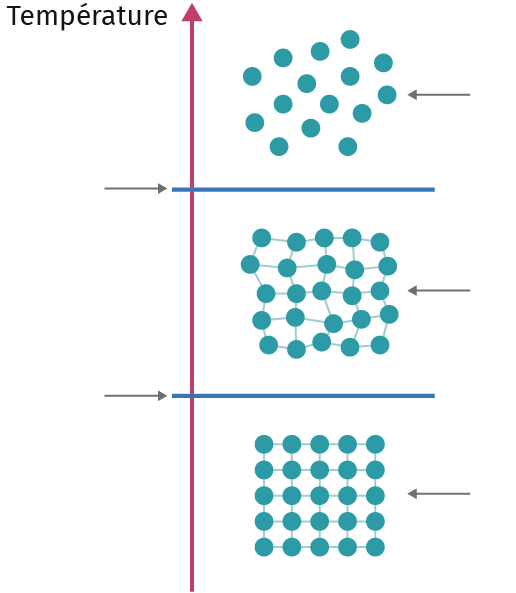
\includegraphics[width=0.6\linewidth]{evaluations/changement_etat.png}
\end{center}

\exo{Un fil de cuivre est :}{0}
\vspace*{-0.3cm}
\begin{qcm}
  \item Un corps pur.
  \item Un mélange.
  \item Une solution.
\end{qcm}
  % %%%% début de la page
\newpage
\enTete{Mouvement et interactions}{2}

\nomPrenomClasse

%%%% titre
\vspace{8pt}
\chevron L'objectif de cette interrogation \textbf{non notée} est d'évaluer où vous en êtes en physique-chimie.

%%%% question
%
\exo{Indiquer l'unité qui correspond à une vitesse.}{0}
\begin{qcm}
  \item Le mètre par seconde (m/s).
  \item Le kilomètre heure (km$\cdot$h).
  \item La seconde par mètre (s/m).
\end{qcm}

%
\exo{Une vitesse instantanée est représentée par une flèche qui porte 3 informations :}{0}
\begin{qcm}
  \item la distance, la direction et la durée.
  \item le sens, l'accélération et le nombre.
  \item la direction, le sens et la valeur.
\end{qcm}

%
\exo{Une observatrice observe depuis le quai un métro roulant à une vitesse constante.
Pour cette observatrice, le mouvement apparent du train est :}{1}

%
\exo{Un observateur est assis dans le métro roulant à une vitesse constante. 
Pour cet observateur, le mouvement apparent du train est :}{1}

%
\exo{Donner la formule de la force de pesanteur, le poids $P$, que l'on ressent sur Terre.}{1}

%
\exo{Indiquer la bonne expression de la force de pesanteur universelle $F_G$ entre deux objets de masse $m_A$ et $m_B$, séparés par une distance $d$.}{0}
\begin{qcm}
  \item $F_G = G \Frac{m_A m_B}{d^2}$
  \item $F_G = G m_A m_B$
  \item $F_G = G \Frac{m_A m_B}{d}$
\end{qcm}

%
\exo{Donner l'unité d'une force.}{1}
  
  %%%% Formative
  % %%%% début de la page
\newpage
\enTete{Corps purs et solutions}{1}

%%%%
\nomPrenomClasse

%%%% evaluation
\vspace*{6pt}
\begin{tableauCompetences}
  \centering RCO --
  Restituer ses connaissances.
  & & & &
  \\ \hline
  %
  \centering APP --
  Extraire une information
  & & & &
  \\ \hline
  %
  \centering REA --
  Réaliser un calcul.
  & & & &
\end{tableauCompetences}


%%%% questions
%
\exo{Un ensemble d'entités chimiques identiques est :\competence{RCO}}{0}
\vspace*{-4pt}
\begin{qcm}
  \item une espèce chimique.
  \item un corps pur.
  \item un mélange.
\end{qcm}

%
\exo{Définir un mélange.\competence{RCO}}{1}

%
\exo{Citer deux liquides \textbf{miscibles}.\competence{RCO}}{1}

%
L'acier doux est un alliage composé de fer (\chemfig{Fe}) et de carbone (\chemfig{C}).
Cet alliage est constitué d'une seule phase.
Un échantillon d'acier de masse $m = 1000 \unit{g}$ comporte une masse de fer $m_{\chemfig{Fe}} = 998 \unit{g}$ et une masse de carbone $m_{\chemfig{C}} = 2,\!00 \unit{g}$

%
\exo{Cet alliage est-il un mélange homogène ou hétérogène ?\competence{APP, RCO}}{1}

%
\exo{Écrire $m_{\chemfig{Fe}}$ et $m_{\chemfig{C}}$ en notation scientifique.\competence{APP, REA}}{1}

%
\exo{Calculer la proportion massique de fer et de carbone dans l'alliage.\competence{APP, REA}}{2}
  % %%%% début de la page
\newpage
\enTete{Corps purs et solutions}{1}

%%%%
\nomPrenomClasse

%%%% evaluation
\vspace*{6pt}
\begin{tableauCompetences}
  \centering RCO --
  Restituer ses connaissances.
  & & & & &
\end{tableauCompetences}


%%%% questions
%
\exo{Un ensemble d'entités chimiques identiques est : }{0}
\begin{qcm}
  \item une espèce chimique.
  \item un corps pur.
  \item un mélange.
\end{qcm}

%
\exo{Définir un mélange.}{1}

%
\vspace*{-12pt}
\exo{Deux liquides sont dits miscibles si ils}{0}
\begin{qcm}
  \item forment un mélange homogène.
  \item forment un mélange hétérogène.
\end{qcm}

%
\exo{Citer deux liquides \textbf{non-miscibles}.}{1}

%
\vspace*{-12pt}
\exo{Donner la formule de la masse volumique, en précisant le sens des symboles utilisés.}{3}

%
\vspace*{-12pt}
\exo{Une solution est :}{0}
\begin{qcm}
  \item Un mélange homogène.
  \item Un mélange hétérogène.
\end{qcm}

%
\exo{Donner le nom d'une solution dont le solvant est l'eau.}{1}

%
\vspace*{-12pt}
\exo{Donner la formule de la concentration massique, en précisant le sens des symboles utilisés.}{3}
  % %%%% début de la page
\newpage
\enTete{Mouvement et interactions}{2}

%%%%
\nomPrenom

%%%% evaluation
\vspace*{6pt}
\begin{tableauCompetences}
  \centering RCO 
  & Restituer ses connaissances.
  & & & &
\end{tableauCompetences}
\vspace*{8pt}

%%%% questions
%
\exo{Indiquer l'unité qui correspond à une vitesse.}{0}
\vspace*{-8pt}
\begin{qcm}
  \item Le mètre par seconde (m/s).
  \item Le kilomètre heure (km$\cdot$h).
\end{qcm}

%
\exo{Une vitesse est représenté par un vecteur qui porte 4 informations :}{0}
\vspace*{-8pt}
\begin{qcm}
  \item la position, la distance, la direction et la durée.
  \item le point, le sens, l'accélération et le nombre.
  \item le point d'application, la direction, le sens et la norme.
\end{qcm}

%
\exo{Une observatrice voit passer un métro roulant à une vitesse constante.
Pour elle le mouvement du métro est :}{1}

%
\exo{Un observateur est assis dans le métro roulant à une vitesse constante. 
Pour lui le mouvement du métro est :}{1}

%
\exo{Donner la formule du vecteur vitesse $\vv{v}_2$ d’un système au point $P_2$ entre les instants $t_1$ et $t_3$ :}{1}
  
  %%%% Fiche réussite
  % \enTeteFicheReussite{Chapitre 1 - Mélange et corps purs}

\begin{tableauConnaissances}
  Je sais la différence entre un corps pur et un mélange.
  & & & Cours p.1-2 & 1,2 p.28
  \\ \hline
  %
  Je connais la formule de la masse volumique $\rho = m/V$.
  Je connais les unités et le sens de ces grandeurs. 
  Je sais calculer un volume, une masse ou une masse volumique avec la formule.
  & & & TP 1 \& 2, cours p.4-6 & 10, 14 p.29
  \\ \hline
  %
  Je sais décrire la composition d'un mélange.
  & & & TP 2, cours p.3-4 & 22, 24 p.31
  \\ \hline
  %
  Je sais identifier un corps pur à partir de données physiques et chimiques qui le caractérisent.
  & & & TP 2 \& 3, cours p.7-8 & 32 p.34
  \\ \hline
  %
  Je sais reconnaître si un échantillon est constitué d'une seule espèce chimique ou s'il s'agit d'un mélange.
  & & & TP 2 \& 3, cours p.7-8 & 31, 32 p.34
  \\ \hline
  %
  Je connais le vocabulaire de la chromatographie sur couche mince : ligne de dépôt, couche mince, éluant, front de l'éluant, etc.
  
  Je sais analyser un chromatogramme.
  & & & TP 3, cours p.8 & 21 p.31
\end{tableauConnaissances}


\basDePageFicheReussite{3}
  % \enTeteFicheReussite{Chapitre 1 - Solutions}
\bigskip

\begin{tableauConnaissances}
  Je sais qu'une solution est un mélange homogène.
  Je sais qu'une solution est composé d'un solvant, l'espèce chimique majoritaire, et de un ou plusieurs solutés.
  & & & TP 4, cours p. 9 & 11 p. 48 \\
  %
  Je sais qu'on parle de solution aqueuse quand le solvant est l'eau.
  & & & TP 4 \& 5, cours p. 9 & \\
  %
  Je connais la formule de la concentration massique $c = m/V$.
  Je connais les unités et le sens de ces grandeurs.
  Je sais calculer une concentration massique, une masse ou un volume avec la formule.
  & & & TP 4 \& 5, cours p. 9, 10 & 14, 15 p. 49 \\
  %
  Je sais ce qu'est une dilution et une dissolution.
  Je connais le protocole pour réaliser une dilution.
  & & & TP 1, 4 \& 5, cours p. 10, 11 & 12, 16 p. 49 \\
  %
  Je sais qu'un dosage est une mesure de concentration.
  Je sais réaliser un dosage par étalonnage, en mesurant une grandeur proportionnelle à la concentration.
  & & & TP 4 \& 5, cours p. 12 & \\
\end{tableauConnaissances}

\basDePageFicheReussite{3}
  % \enTeteFicheReussite{Chapitre 2 - \sndChapitreDeux}
\bigskip

\begin{tableauConnaissances}
  % 
  Je sais que le mouvement dépend du référentiel choisi et je connais le modèle du point matériel.
  & & & Activité 1, 2 \& 3, cours p. 1-4 & 11, 13 p. 210
  \\ \hline 
  %
  Je sais décrire le mouvement d'un système (trajectoire + évolution de son vecteur vitesse). Je sais reconnaitre un mouvement rectiligne uniforme.
  & & &  Activité 1, 2 \& 3, cours p. 1-4 & 11, 14 p.210-211
  \\ \hline
  %
  Je sais calculer et tracer un vecteur vitesse à partir du vecteur déplacement et de l'écart de temps entre deux positions. 
  & & & Activité 3 \& 7, cours p. 1-4 & 14, 16 p. 211, 11 p. 243
  \\ \hline
  %
  Je sais qu'une force s'exprime en newton (N) et je sais représenter une force en terme de vecteurs, en faisant attention à son point d'application.
  & & & Activité 4 \& 5, cours p. 6-8 & 15, 16 p. 228, 10 p. 243 
  \\ \hline
  %
  Je connais les caractéristiques des forces suivantes : poids, réaction du support et forces de frottements.
  & & & Activité 4 \& 5, cours p. 6-8 & 11, 14, 17 p. 227-228
  \\ \hline
  %
  Je sais utiliser le principe d'inertie et sa contraposée pour relier le mouvement d'un système au forces qui s'exercent sur lui.
  & & & Activité 5, 6, 7 \& 8, cours p. 9-10 & 10, 11 p.243
  %
\end{tableauConnaissances}

\basDePageFicheReussite{2}
  % \enTeteFicheReussite{Chapitre 3 - Atome et ordre de grandeur}
\bigskip

\begin{tableauConnaissances}
  % 
  Je sais calculer et utiliser les puissances de dix.
  Je sais utiliser la notation scientifique.
  Je sais calculer un ordre de grandeur avec les puissances de dix.
  & & &  Activité 1 & Exercice 15, 16 \& 27 p. 81
  \\ \hline
  %
  Je sais que la masse d’un atome est essentiellement contenue dans celle de son noyau.
  Je sais que le noyau est très petit devant la taille de l'atome.
  & & & Activité 2 & Exercice 9, 13 p. 81
  \\ \hline
  %
  Je connais les charges électriques des électrons, neutrons et protons.
  J'ai compris pourquoi l'atome a une charge globale neutre.
  & & & Activité 2 \& 3 &
  \\ \hline
  %
  Je connais les composants d'un atome et de son noyau. 
  Je sais faire la différence entre électrons, protons, neutrons et nucléons.
  & & & Activité 3 &
  \\ \hline
  %
  Je peux déterminer la composition d'un atome à partir de sa notation symbolique \isotope{A}{Z}{X} et inversement.
  & & & Activité 3 & Exercice 7, 13 p. 81 
  \\ \hline
  %
  Je sais faire la différence entre les termes atome, ion, isotope.
  & & & Activité 3 & 
  \\ \hline
  %
  Je sais que la description d'un atome est un modèle, dont l'évolution dépend d'observations expérimentales.
  & & & Activité 4 & Doc. p. 105
  %
\end{tableauConnaissances}

\basDePageFicheReussite
\bigskip

\coursFicheReussite
  % \enTeteFicheReussite{Chapitre 3 - Cortège électronique, ions, molécules}
\bigskip

\begin{tableauConnaissances}
  %
  %Je sais que les électrons se structurent en couche (1, 2, 3) et sous-couche (s, p) autour du noyau.
  Je peux écrire la configuration électronique d'un atome en remplissant les sous-couches s et p dans le bon ordre.
  & & & Activité 5, 6 &
  \\ \hline
  %
  Je sais que les éléments chimiques sont rangées par colonne (famille) et par ligne (période) dans le tableau périodique.
  & & & Activité 6 &
  \\ \hline
  %
  Je peux identifier la couche externe d'un atome et combien d'électrons de valence s'y trouvent.
  & & & Activité 5, 6, 7, 8 &
  \\ \hline
  %
  Je sais repérer la famille des gaz nobles dans le tableau périodique.
  Je sais que leur couche externe pleine les rend très stables.
  & & & Activité 6, 7, 8 &
  \\ \hline
  %
  Je connais la règle du duet et de l'octet.
  Je peux les appliquer pour trouver quel ion stable peut être formé à partir d'un atome.
  & & & Activité 7 &
  \\ \hline
  %
  Je sais que les molécules sont composées d'atomes.
  Je sais que la stabilité d'une molécule est due aux électrons de valence partagés entre les atomes.
  & & & Activité 8 &
  \\ \hline
  %
  Je peux analyser un schéma de Lewis pour expliquer la stabilité d'une molécule.
  & & & Activité 8 &
  \\ \hline
  %
  Je sais qu'une espèce chimique est constitué d'un très grand nombre d'entités chimiques.
  Je sais ce que représente une mole.
  & & & Activité 9 &
  %
  %
\end{tableauConnaissances}

\basDePageFicheReussite
\bigskip

\coursFicheReussite
  % \enTeteFicheReussite{Chapitre 4 - Ondes lumineuses et optique}
\bigskip

\begin{tableauConnaissancesSansExercices}
  %
  Je sais que la lumière est une onde électromagnétique.
  Je sais que la lumière peut être monochromatique ou polychromatique.
  & & & Activité 1
  \\ \hline
  %
  Je connais les deux types de spectre d'émission et je sais les reconnaître.
  & & & TP 1
  \\ \hline
  %
  Je sais qu'un corps chaud produit un spectre continu.
  Les propriétés de ce spectre dépendent de la température du corps chaud.
  & & & TP 1
  \\ \hline
  %
  Je sais qu'un gaz atomique ou moléculaire excité produit un spectre de raies.
  Je sais que chaque élément chimique possède son propre spectre de raies qui permet de le reconnaître.
  & & & TP 1, activité 2
  \\ \hline
  %
  Je sais repérer une raie sur un spectre en mesurant sa longueur d'onde.
  & & & TP 1, activité 2
  \\ \hline
  %
  Je connais le vocabulaire de la réfraction et je sais lire les angles d'incidence et de réfraction à partir d'un schéma.
  & & & TP 2, activité 4
  \\ \hline
  %
  Je sais appliquer la loi de Snell-Descartes pour calculer un indice de réfraction ou un angle.
  & & & TP 2, activité 4
  \\ \hline
  %
  Je sais expliquer comment l'oeil parvient à faire l'image d'un objet.
  & & & Activité 3
  \\ \hline
  %
  Je sais expliquer comment fonctionne une lentille convergente et je connais le vocabulaire pour la décrire (foyer image, foyer objet, centre optique).
  & & & TP 3, activité 3
  \\ \hline
  %
  Je connais la formule du grandissement et je sais l'appliquer pour calculer la taille d'un objet ou d'une image.
  & & & TP 3, Activité 3
  \\ \hline
  %
  Je sais expliquer pourquoi la lumière blanche est dispersée après avoir traversé un prisme.
  & & & Activité 4
  %
\end{tableauConnaissancesSansExercices}
\bigskip 

% \basDePageFicheReussite
% \coursFicheReussite
\questionFicheReussite{2}
  
  %%%% Compétences
  % %\newpage
\pasDePagination

%%%% liste des compétences
\titre{Liste des compétences évaluées}

Ce tableau liste l'ensemble des compétences évaluées au cours de l'année.
Ces compétences sont liées à la méthode scientifique : chaque compétence représente une étape nécessaire pour étudier une situation nouvelle en appliquant la méthode scientifique.
Pour chaque compétence, des exemples de capacités concrètes sont présentées.
\bigskip

L'objectif de cette liste est de vous aider à identifier ce qui est attendu de vous au cours de l'année.
\bigskip

Au début de chaque évaluation, les compétences effectivement évaluées seront présentées clairement. 
\bigskip

\begin{tabularx}{\linewidth}{| m{0.2\linewidth} | X |}
  \hline
  \rowcolor{gray!20} 
  \centering \textbf{Compétences} & \textbf{Capacités associées}
  \\ \hline
  %
  \centering Restituer ses connaissances (RCO) &
  -- Énoncer les définitions du cours. \newline
  -- Énoncer des exemples courants présentés en cours
  \\ \hline
  %
  \centering S'approprier (APP) &
  -- Énoncer un problème à résoudre (problématique). \newline
  -- Rechercher et organiser l'information. \newline
  -- Représenter la situation par un schéma.
  \\ \hline
  %
  \centering Analyser/ Raisonner (ANA/RAI) &
  -- Formuler des hypothèses. \newline
  -- Proposer une stratégie de résolution. \newline
  -- Évaluer des ordres de grandeurs. \newline
  -- Choisir un modèle ou des lois pertinentes. \newline
  -- Choisir, élaborer, justifier un protocole. \newline
  -- Prévoir à l'aide d'un modèle. \newline
  -- Procéder à des analogies.
  \\ \hline
  %
  \centering Réaliser (REA) &
  -- Mettre en \oe{}uvre les étapes d'une démarche. \newline
  -- Utiliser un modèle. \newline
  -- Calculer, représenter, collecter des données, etc. \newline
  -- Mettre en \oe{}uvre un protocole expérimental en respectant les règles de sécurités.
  \\ \hline
  %
  \centering Valider (VAL) & 
  -- Faire preuve d'esprit critique. \newline
  -- Identifier des sources d'erreur, estimer une incertitude .\newline
  -- Comparer avec des valeurs de références. \newline
  -- Confronter un modèle à des résultats expérimentaux. \newline
  -- Proposer des améliorations de la démarche ou du modèle.
  \\ \hline
  %
  \centering Communiquer (COM) &
  -- Présenter de manière argumentée, synthétique et cohérente. \newline
  -- Utiliser un vocabulaire ou une représentation adaptée. \newline
  -- Échanger entre élèves.
  \\ \hline
\end{tabularx}
  % \newcommand{\competenceClasseur}{
  \begin{center}
    \setlength{\extrarowheight}{6pt}
    \begin{tabular}{| l | c | c | c | c |}
      \hline
      \rowcolor{gray!20} 
      %
      \textbf{Items évalués} & D & C & B & A
      \\ \hline
      %
      Propreté  & & & &
      \\ \hline
      %
      Rangement (feuilles dans le bon ordre) & & & &
      \\ \hline
      %
      Complétion (feuilles présentes \textit{et} remplies) & & & & 
      \\ \hline
    \end{tabular}
  \end{center}
}

\pasDePagination

\competenceClasseur
\bigskip
\competenceClasseur
\bigskip
\competenceClasseur
\bigskip
\competenceClasseur
\bigskip
\competenceClasseur
\end{document}